\chapter{Random Variables}

%% Introduction %%%%%%%%%%%%%%%%%%%%%%%%%%%%%%%%%%%%%%%%%%%%%%%%%%%%%%%%%%%%%%%
So far we focused on probabilities of \idx{events} ---that you win the
Monty Hall game; that you have a rare medical condition, given that you
tested positive; \dots.  Now we focus on quantitative questions: \emph{How
  many} contestants must play the Monty Hall game until one of them
finally wins? \dots {\em How long} will this condition last?  {\em How
  much} will I lose playing 6.042 games all day?  Random variables are the
mathematical tool for addressing such questions.


%% Random Variables %%%%%%%%%%%%%%%%%%%%%%%%%%%%%%%%%%%%%%%%%%%%%%%%%%%%%%%%%%%
\hyperdef{random}{vars}{\section{Random Variable Examples}}\label{ran_var_examples_sec}

\begin{definition}
  A \term{random variable}, $R$, on a probability space is a function whose
  domain is the sample space.
\end{definition}
The codomain of $R$ can be anything, but will usually be a subset of the
real numbers.  Notice that the name ``random variable'' is a misnomer;
random variables are actually functions!

For example, suppose we toss three independent, unbiased coins.  Let $C$
be the number of heads that appear.  Let $M = 1$ if the three coins come
up all heads or all tails, and let $M = 0$ otherwise.  Now every outcome
of the three coin flips uniquely determines the values of $C$ and $M$.
For example, if we flip heads, tails, heads, then $C = 2$ and $M = 0$.  If
we flip tails, tails, tails, then $C = 0$ and $M = 1$.  In effect, $C$
counts the number of heads, and $M$ indicates whether all the coins match.

Since each outcome uniquely determines $C$ and $M$, we can regard them
as functions mapping outcomes to numbers.  For this experiment, the
sample space is:
\begin{eqnarray*}
\sspace & = & \set{ HHH, HHT, HTH, HTT, THH, THT, TTH, TTT }.
\end{eqnarray*}
Now $C$ is a function that maps each outcome in the sample space to a 
number as follows:
\[
\begin{array}{rclcrcl}
C(HHH) & = & 3 & \quad & C(THH) & = & 2 \\
C(HHT) & = & 2 & \quad & C(THT) & = & 1 \\
C(HTH) & = & 2 & \quad & C(TTH) & = & 1 \\
C(HTT) & = & 1 & \quad & C(TTT) & = & 0.
\end{array}
\]
Similarly, $M$ is a function mapping each outcome another way:
\[
\begin{array}{rclcrcl}
M(HHH) & = & 1 & \quad & M(THH) & = & 0 \\
M(HHT) & = & 0 & \quad & M(THT) & = & 0 \\
M(HTH) & = & 0 & \quad & M(TTH) & = & 0 \\
M(HTT) & = & 0 & \quad & M(TTT) & = & 1.
\end{array}
\]
So $C$ and $M$ are \idx{random variables}.

\subsection{Indicator Random Variables}

An \term{indicator random variable} is a random variable that maps every
outcome to either 0 or 1.  These are also called \term{Bernoulli
  variables}.  The random variable $M$ is an example.  If all three coins
match, then $M=1$; otherwise, $M = 0$.

Indicator random variables are closely related to events.  In
particular, an indicator partitions the sample space into those
outcomes mapped to 1 and those outcomes mapped to 0.  For example, the
indicator $M$ partitions the sample space into two blocks as follows:
\[
\underbrace{HHH \quad TTT}_{\text{$M = 1$}} \quad
\underbrace{HHT \quad HTH \quad HTT \quad
        THH \quad THT \quad TTH}_{\text{$M = 0$}}.
\]

In the same way, an event, $E$, partitions the sample space into those
outcomes in $E$ and those not in $E$.  So $E$ is naturally associated with
an indicator random variable, \index{$I_E$, indicator for event $E$}
$I_E$, where $I_E(p) = 1$ for outcomes $p \in E$ and $I_E(p) = 0$ for
outcomes $p \notin E$.  Thus, $M=I_F$ where $F$ is the event that all
three coins match.

\subsection{Random Variables and Events}

There is a strong relationship between events and more general random
variables as well.  A random variable that takes on several values
partitions the sample space into several blocks.  For example, $C$
partitions the sample space as follows:
\[
\underbrace{TTT}_{\text{$C = 0$}} \quad
\underbrace{TTH \quad THT \quad HTT}_{\text{$C = 1$}} \quad
\underbrace{THH \quad HTH \quad HHT}_{\text{$C = 2$}} \quad
\underbrace{HHH}_{\text{$C = 3$}}.
\]
Each block is a subset of the sample space and is therefore
an event.  Thus, we can regard an equation or inequality involving a
random variable as an event.  For example, the event that $C = 2$
consists of the outcomes $THH$, $HTH$, and $HHT$.  The event $C \leq
1$ consists of the outcomes $TTT$, $TTH$, $THT$, and $HTT$.

Naturally enough, we can talk about the probability of events defined
by properties of random variables.  For example, 
\begin{eqnarray*}
\pr{C = 2}
        & = &   \pr{THH} + \pr{HTH} + \pr{HHT} \\
        & = &   \frac{1}{8} + \frac{1}{8} + \frac{1}{8} =  \frac{3}{8}.
\end{eqnarray*}

\iffalse
As another example:
\begin{eqnarray*}
\pr{M = 1}
        & = &   \pr{TTT} + \pr{HHH}\\
        & = &   \frac{1}{8} + \frac{1}{8} =    \frac{1}{4}.
\end{eqnarray*}

\subsection{Conditional Probability}

Mixing conditional probabilities and events involving random variables
creates no new difficulties.  For example, $\prcond{C \geq 2}{M = 0}$
is the probability that at least two coins are heads ($C \geq 2$),
given that not all three coins are the same ($M = 0$).  We can compute
this probability using the definition of conditional probability:
\begin{eqnarray*}
\prcond{C \geq 2}{M = 0}
        & = &   \frac{\pr{[C \geq 2] \intersect [M = 0]}}{\pr{M = 0}} \\
        & = &   \frac{\pr{\set{THH, HTH, HHT}}}
                        {\pr{\set{THH, HTH, HHT, HTT, THT, TTH }}} \\
        & = &   \frac{3/8}{6/8} = \frac{1}{2}.
\end{eqnarray*}
The expression $[C \geq 2] \intersect [M = 0]$ on the first line may look odd;
what is the set operation $\intersect$ doing between an inequality and an
equality?  But recall that, in this context, $[C \geq 2]$ and $[M = 0]$
are \emph{events}, namely, \emph{sets} of outcomes.
\fi

\subsection{Independence}

The notion of independence carries over from events to random variables as
well.  Random variables $R_1$ and $R_2$ are \index{independent random
  variables} \emph{independent} iff for all $x_1$ in the codomain of
$R_1$, and $x_2$ in the codomain of $R_2$, we have:
\[
\pr{R_1 = x_1 \QAND R_2 = x_2}  =  \pr{R_1 = x_1} \cdot \pr{R_2 = x_2}.
\]
As with events, we can formulate independence for random
variables in an equivalent and perhaps more intuitive way: random
variables $R_1$ and $R_2$ are independent if for all $x_1$ and $x_2$
\[
\prcond{R_1 = x_1}{R_2 = x_2}  =  \pr{R_1 = x_1}.
\]
whenever the lefthand conditional probability is defined, that is,
whenever $\pr{R_2 = x_2} > 0$.

As an example, are $C$ and $M$ independent?  Intuitively, the answer
should be ``no''.  The number of heads, $C$, completely determines
whether all three coins match; that is, whether $M = 1$.  But, to
verify this intuition, we must find some $x_1, x_2 \in \reals$
such that:
\[
\pr{C = x_1 \QAND M = x_2} \neq \pr{C = x_1} \cdot \pr{M = x_2}.
\]
One appropriate choice of values is $x_1 = 2$ and $x_2 = 1$.
In this case, we have:
\[
\pr{C = 2 \QAND M = 1} = 0 \neq \dfrac{1}{4} \cdot \dfrac{3}{8} = \pr{M
= 1} \cdot \pr{C = 2}.
\]
The first probability is zero because we never have exactly two heads ($C
= 2$) when all three coins match ($M = 1$).  The other two probabilities
were computed earlier.

On the other hand, let $H_1$ be the indicator variable for event that the
first flip is a Head, so
\[
[H_1 = 1] = \set{HHH, HTH, HHT, HTT}.
\]
Then $H_1$ is independent of $M$, since
\begin{align*}
\pr{M=1} & = 1/4 = \prcond{M=1}{H_1=1} = \prcond{M=1}{H_1=0}\\
\pr{M=0} & = 3/4 = \prcond{M=0}{H_1=1} = \prcond{M=0}{H_1=0}
\end{align*}
This example is an instance of a simple lemma:
\begin{lemma}
  Two events are independent iff their \idx{indicator variables} are
  independent.
\end{lemma}
As with events, the notion of independence generalizes to more than two
random variables.
\begin{definition}
Random variables $R_1, R_2, \dots, R_n$ are \term{mutually independent} iff
\begin{eqnarray*}
\lefteqn{\pr{R_1 = x_1 \QAND R_2 = x_2 \QAND \cdots \QAND R_n = x_n}}\\
        & = & \pr{R_1 = x_1} \cdot \pr{R_2 = x_2} \cdots \pr{R_n = x_n}.
\end{eqnarray*}
for all $x_1, x_2, \dots, x_n$.
\end{definition}

It is a simple exercise to show that the probability that any
\emph{subset} of the variables takes a particular set of values is equal
to the product of the probabilities that the individual variables take
their values.  Thus, for example, if $R_1, R_2, \dots, R_{100}$ are
mutually independent random variables, then it follows that:
\[
\pr{R_1 = 7 \QAND R_7 = 9.1 \QAND R_{23} = \pi} = \pr{R_1 = 7} \cdot
\pr{R_7 = 9.1} \cdot \pr{R_{23} = \pi}.
\]

%% Random Variables Problems %%%%%%%%%%%%%%%%%%%%%%%%%%%%%%%%%%%%%%%%%%%%%%%%%%
%\startclassproblems

%% Probability Distributions %%%%%%%%%%%%%%%%%%%%%%%%%%%%%%%%%%%%%%%%%%%%%%%%%%
\section{Probability Distributions}\label{distributions_sec}

A random variable maps outcomes to values, but random variables that show
up for different spaces of outcomes wind up behaving in much the same way
because they have the same probability of taking any given value.  Namely,
random variables on different probability spaces may wind up having the
same probability density function.

\begin{definition}
Let $R$ be a random variable with with codomain $V$.
The \term{probability density function (pdf)} of $R$
is a function $\pdf_R : V \to [0,1]$ defined by:
%
\[
\pdf_R(x) \eqdef \begin{cases}
            \pr{R = x} & \text{if } x \in \range{R},\\
             0 & \text{if } x \notin \range{R}.
           \end{cases}
\]
\end{definition}
%
A consequence of this definition is that
%
\[
\sum_{x \in \range{R}} \pdf_R(x) = 1.
\]
This follows because $R$ has a value for each outcome, so summing the
probabilities over all outcomes is the same as summing over the
probabilities of each value in the range of $R$.

As an example, let's return to the experiment of rolling two fair,
independent dice.  As before, let $T$ be the total of the two rolls.
This random variable takes on values in the set $V = \set{2, 3,
\dots, 12}$.  A plot of the probability density function is shown
below:
%
\begin{center}
\begin{picture}(305,110)(-75,-40)
%\put(-75,-40){\dashbox(305,110)} % bounding box
\put(0,0){\vector(1,0){230}}
\put(0,0){\vector(0,1){70}}
\put(-1,60){\line(1,0){2}}
\put(-15,60){\makebox(0,0){{\small $6/36$}}}
\put(-1,30){\line(1,0){2}}
\put(-15,30){\makebox(0,0){{\small $3/36$}}}
\put(-50,40){\makebox(0,0){$\pdf_R(x)$}}
\put(120,-30){\makebox(0,0){$x \in V$}}
\put(0,0){\framebox(20,10){}}
\put(10,-10){\makebox(0,0){2}}
\put(20,0){\framebox(20,20){}}
\put(30,-10){\makebox(0,0){3}}
\put(40,0){\framebox(20,30){}}
\put(50,-10){\makebox(0,0){4}}
\put(60,0){\framebox(20,40){}}
\put(70,-10){\makebox(0,0){5}}
\put(80,0){\framebox(20,50){}}
\put(90,-10){\makebox(0,0){6}}
\put(100,0){\framebox(20,60){}}
\put(110,-10){\makebox(0,0){7}}
\put(120,0){\framebox(20,50){}}
\put(130,-10){\makebox(0,0){8}}
\put(140,0){\framebox(20,40){}}
\put(150,-10){\makebox(0,0){9}}
\put(160,0){\framebox(20,30){}}
\put(170,-10){\makebox(0,0){10}}
\put(180,0){\framebox(20,20){}}
\put(190,-10){\makebox(0,0){11}}
\put(200,0){\framebox(20,10){}}
\put(210,-10){\makebox(0,0){12}}
\end{picture}
\end{center}
%
The lump in the middle indicates that sums close to 7 are the most
likely.  The total area of all the rectangles is 1 since the dice must
take on exactly one of the sums in $V = \set{2, 3, \dots, 12}$.

A closely-related idea is the \term{cumulative distribution function
(cdf)} for a random variable $R$ whose codomain is real numbers.  This is a
function $\cdf_R : \reals \to [0,1]$ defined by:
%
\[
\cdf_R(x) = \pr{R \leq x}
\]
%
As an example, the cumulative distribution function for the random
variable $T$ is shown below:
%
\begin{center}
\begin{picture}(305,155)(-75,-40)
%\put(-75,-40){\dashbox(305,155)} % bounding box
\put(0,0){\vector(1,0){230}}
\put(0,0){\vector(0,1){115}}
\put(-1,108){\line(1,0){2}}
\put(-15,108){\makebox(0,0){{\small $1$}}}
\put(-1,54){\line(1,0){2}}
\put(-15,54){\makebox(0,0){{\small $1/2$}}}
\put(-15,0){\makebox(0,0){{\small $0$}}}
\put(-50,81){\makebox(0,0){$\cdf_R(x)$}}
\put(120,-30){\makebox(0,0){$x \in V$}}
\put(0,0){\framebox(20,3){}}
\put(10,-10){\makebox(0,0){2}}
\put(20,0){\framebox(20,9){}}
\put(30,-10){\makebox(0,0){3}}
\put(40,0){\framebox(20,18){}}
\put(50,-10){\makebox(0,0){4}}
\put(60,0){\framebox(20,30){}}
\put(70,-10){\makebox(0,0){5}}
\put(80,0){\framebox(20,45){}}
\put(90,-10){\makebox(0,0){6}}
\put(100,0){\framebox(20,63){}}
\put(110,-10){\makebox(0,0){7}}
\put(120,0){\framebox(20,78){}}
\put(130,-10){\makebox(0,0){8}}
\put(140,0){\framebox(20,90){}}
\put(150,-10){\makebox(0,0){9}}
\put(160,0){\framebox(20,99){}}
\put(170,-10){\makebox(0,0){10}}
\put(180,0){\framebox(20,105){}}
\put(190,-10){\makebox(0,0){11}}
\put(200,0){\framebox(20,108){}}
\put(210,-10){\makebox(0,0){12}}
\end{picture}
\end{center}
%
The height of the $i$-th bar in the cumulative distribution function
is equal to the \textit{sum} of the heights of the leftmost $i$ bars
in the probability density function.  This follows from the
definitions of pdf and cdf:
%
\begin{align*}
\cdf_R(x) & = \pr{R \leq x} \\
          & = \sum_{y \leq x} \pr{R = y} \\
          & = \sum_{y \leq x} \pdf_R(y)
\end{align*}

In summary, $\pdf_R(x)$ measures the probability that $R = x$ and
$\cdf_R(x)$ measures the probability that $R \leq x$.  Both the
$\pdf_R$ and $\cdf_R$ capture the same information about the random
variable $R$--- you can derive one from the other ---but sometimes one
is more convenient.  The key point here is that neither the
probability density function nor the cumulative distribution function
involves the sample space of an experiment.

\iffalse
Thus, through these
functions, we can study random variables without reference to a
particular experiment.
\fi

We'll now look at three important distributions and some applications.

\subsection{Bernoulli Distribution}

\index{indicator variable} Indicator random variables are perhaps the most
common type because of their close association with events.  The
probability density function of an indicator random variable, $B$, is
always
%
\begin{align*}
\pdf_B(0) & = p \\
\pdf_B(1) & = 1 - p \\
\end{align*}
%
where $0 \leq p \leq 1$.  The corresponding cumulative distribution
function is:
%
\begin{align*}
\cdf_B(0) & = p \\
\cdf_B(1) & = 1
\end{align*}
%
%This is called the \term{Bernoulli distribution}. 
%The number of heads
%flipped on a (possibly biased) coin has a Bernoulli distribution.

\subsection{Uniform Distribution}

A random variable that takes on each possible value with the same
probability is called \term{uniform}.  For example, the probability
density function of a random variable $U$ that is uniform on the set
$\set{1, 2, \dots, N}$ is:
%
\begin{align*}
\pdf_U(k) = \frac{1}{N}
\end{align*}
%
And the cumulative distribution function is:
%
\begin{align*}
\cdf_U(k) = \frac{k}{N}
\end{align*}
%
Uniform distributions come up all the time.  For example, the number
rolled on a fair die is uniform on the set $\set{1, 2, \dots, 6}$.

\subsection{The Numbers Game}\label{bigger_number_subsec}

Let's play a game!  I have two envelopes.  Each contains an integer in
the range $0, 1, \dots, 100$, and the numbers are distinct.  To win
the game, you must determine which envelope contains the larger
number.  To give you a fighting chance, I'll let you peek at the
number in one envelope selected at random.  Can you devise a strategy
that gives you a better than 50\% chance of winning?

For example, you could just pick an evelope at random and guess that
it contains the larger number.  But this strategy wins only 50\% of
the time.  Your challenge is to do better.

So you might try to be more clever.  Suppose you peek in the left
envelope and see the number 12.  Since 12 is a small number, you might
guess that that other number is larger.  But perhaps I'm sort of
tricky and put small numbers in \textit{both} envelopes.  Then your
guess might not be so good!

An important point here is that the numbers in the envelopes may
\textit{not} be random.  I'm picking the numbers and I'm choosing them
in a way that I think will defeat your guessing strategy.  I'll only
use randomization to choose the numbers if that serves \textit{my}
end:  making you lose!

\subsubsection{Intuition Behind the Winning Strategy}

Amazingly, there is a strategy that wins more than 50\% of the time,
regardless of what numbers I put in the envelopes!

Suppose that you somehow knew a number $x$ \textit{between} my lower
number and higher numbers.  Now you peek in an envelope and see one or
the other.  If it is bigger than $x$, then you know you're peeking at
the higher number.  If it is smaller than $x$, then you're peeking at
the lower number.  In other words, if you know a number $x$ between
my lower and higher numbers, then you are certain to win the game.

The only flaw with this brilliant strategy is that you do \textit{not}
know $x$.  Oh well.

But what if you try to \textit{guess} $x$?  There is some probability
that you guess correctly.  In this case, you win 100\% of the time.
On the other hand, if you guess incorrectly, then you're no worse off
than before; your chance of winning is still 50\%.  Combining these
two cases, your overall chance of winning is better than 50\%!

Informal arguments about probability, like this one, often sound
plausible, but do not hold up under close scrutiny.  In contrast, this
argument sounds completely implausible--- but is actually correct!

\subsubsection{Analysis of the Winning Strategy}

For generality, suppose that I can choose numbers from the set
$\set{0, 1, \dots, n}$.  Call the lower number $L$ and the higher
number $H$.

Your goal is to guess a number $x$ between $L$ and $H$.  To avoid
confusing equality cases, you select $x$ at random from among the
half-integers:
%
\[
\set{\frac{1}{2},\ 1\frac{1}{2},\ 2\frac{1}{2},\ \dots,\ n - \frac{1}{2}}
\]
%
But what probability distribution should you use?

The uniform distribution turns out to be your best bet.  An informal
justification is that if I figured out that you were unlikely to pick
some number--- say $50\frac{1}{2}$--- then I'd always put 50 and 51 in
the evelopes.  Then you'd be unlikely to pick an $x$ between $L$ and
$H$ and would have less chance of winning.

After you've selected the number $x$, you peek into an envelope and
see some number $p$.  If $p > x$, then you guess that you're looking
at the larger number.  If $p < x$, then you guess that the other
number is larger.

All that remains is to determine the probability that this strategy
succeeds.  We can do this with the usual four step method and a tree
diagram.

\noindent \textbf{Step 1: Find the sample space. }  You either choose
$x$ too low ($< L$), too high ($> H$), or just right ($L < x < H$).
Then you either peek at the lower number ($p = L$) or the higher
number ($p = H$).  This gives a total of six possible outcomes.
%
\begin{center}
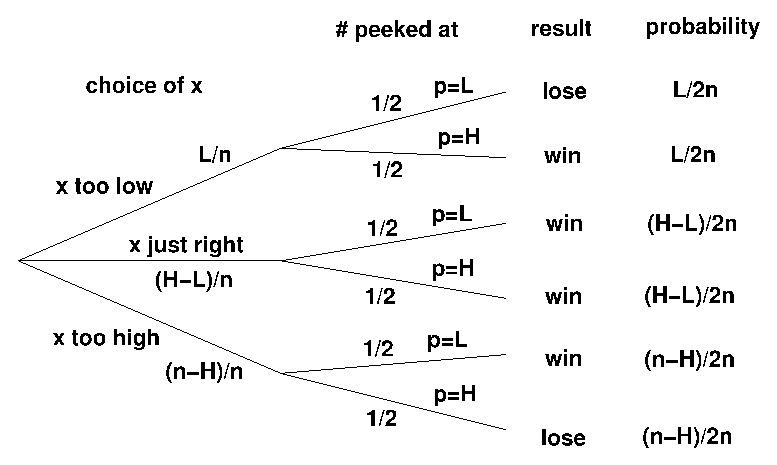
\includegraphics[height=2.5in]{figures/numbers-game}
\end{center}

\noindent \textbf{Step 2: Define events of interest. } The four
outcomes in the event that you win are marked in the tree diagram.

\noindent \textbf{Step 3: Assign outcome probabilities. } First, we
assign edge probabilities.  Your guess $x$ is too low with probability
$L/n$, too high with probability $(n-H)/n$, and just right with
probability $(H-L)/n$.  Next, you peek at either the lower or higher
number with equal probability.  Multiplying along root-to-leaf paths
gives the outcome probabilities.

\noindent \textbf{Step 4: Compute event probabilities. }  The
probability of the event that you win is the sum of the probabilities
of the four outcomes in that event:
%
\begin{align*}
\pr{\text{win}}
    & = \frac{L}{2n} + \frac{H-L}{2n} + \frac{H-L}{2n}  + \frac{n-H}{2n} \\
    & = \frac{1}{2} + \frac{H-L}{2n} \\
    & \geq \frac{1}{2} + \frac{1}{2n}
\end{align*}
%
The final inequality relies on the fact that the higher number $H$ is
at least 1 greater than the lower number $L$ since they are required
to be distinct.

Sure enough, you win with this strategy more than half the time,
regardless of the numbers in the envelopes!  For example, if I choose
numbers in the range $0, 1, \dots, 100$, then you win with probability at
least $\frac{1}{2} + \frac{1}{200} = 50.5\%$.  Even better, if I'm allowed
only numbers in the range $0, \dots, 10$, then your probability of
winning rises to 55\%!  By Las Vegas standards, those are great odds!


\subsection{Binomial Distribution}\label{binomial_distribution_section}

The \term{binomial distribution} plays an important role in Computer
Science as it does in most other sciences.  The standard example of a
random variable with a binomial distribution is the number of heads that
come up in $n$ independent flips of a coin; call this random variable
$H_n$.  If the coin is fair, then $H_n$ has an \textit{unbiased binomial
  density function}:
%
\[
\pdf_{H_n}(k) = \binom{n}{k} 2^{-n}.
\]
%
This follows because there are $\binom{n}{k}$ sequences of $n$ coin
tosses with exactly $k$ heads, and each such sequence has probability
$2^{-n}$.

Here is a plot of the unbiased probability density function
$\pdf_{H_n}(k)$ corresponding to $n = 20$ coins flips.  The most likely
outcome is $k = 10$ heads, and the probability falls off rapidly for
larger and smaller values of $k$.  These falloff regions to the left and
right of the main hump are usually called the \term{tails of the
distribution}.
%
\begin{center}
% GNUPLOT: LaTeX picture
\setlength{\unitlength}{0.240900pt}
\ifx\plotpoint\undefined\newsavebox{\plotpoint}\fi
\sbox{\plotpoint}{\rule[-0.200pt]{0.400pt}{0.400pt}}%
\begin{picture}(1500,900)(0,0)
\font\gnuplot=cmr10 at 10pt
\gnuplot
\sbox{\plotpoint}{\rule[-0.200pt]{0.400pt}{0.400pt}}%
\put(140.0,82.0){\rule[-0.200pt]{4.818pt}{0.400pt}}
\put(120,82){\makebox(0,0)[r]{0}}
\put(1419.0,82.0){\rule[-0.200pt]{4.818pt}{0.400pt}}
\put(140.0,168.0){\rule[-0.200pt]{4.818pt}{0.400pt}}
\put(120,168){\makebox(0,0)[r]{0.02}}
\put(1419.0,168.0){\rule[-0.200pt]{4.818pt}{0.400pt}}
\put(140.0,255.0){\rule[-0.200pt]{4.818pt}{0.400pt}}
\put(120,255){\makebox(0,0)[r]{0.04}}
\put(1419.0,255.0){\rule[-0.200pt]{4.818pt}{0.400pt}}
\put(140.0,341.0){\rule[-0.200pt]{4.818pt}{0.400pt}}
\put(120,341){\makebox(0,0)[r]{0.06}}
\put(1419.0,341.0){\rule[-0.200pt]{4.818pt}{0.400pt}}
\put(140.0,428.0){\rule[-0.200pt]{4.818pt}{0.400pt}}
\put(120,428){\makebox(0,0)[r]{0.08}}
\put(1419.0,428.0){\rule[-0.200pt]{4.818pt}{0.400pt}}
\put(140.0,514.0){\rule[-0.200pt]{4.818pt}{0.400pt}}
\put(120,514){\makebox(0,0)[r]{0.1}}
\put(1419.0,514.0){\rule[-0.200pt]{4.818pt}{0.400pt}}
\put(140.0,601.0){\rule[-0.200pt]{4.818pt}{0.400pt}}
\put(120,601){\makebox(0,0)[r]{0.12}}
\put(1419.0,601.0){\rule[-0.200pt]{4.818pt}{0.400pt}}
\put(140.0,687.0){\rule[-0.200pt]{4.818pt}{0.400pt}}
\put(120,687){\makebox(0,0)[r]{0.14}}
\put(1419.0,687.0){\rule[-0.200pt]{4.818pt}{0.400pt}}
\put(140.0,774.0){\rule[-0.200pt]{4.818pt}{0.400pt}}
\put(120,774){\makebox(0,0)[r]{0.16}}
\put(1419.0,774.0){\rule[-0.200pt]{4.818pt}{0.400pt}}
\put(140.0,860.0){\rule[-0.200pt]{4.818pt}{0.400pt}}
\put(120,860){\makebox(0,0)[r]{0.18}}
\put(1419.0,860.0){\rule[-0.200pt]{4.818pt}{0.400pt}}
\put(140.0,82.0){\rule[-0.200pt]{0.400pt}{4.818pt}}
\put(140,41){\makebox(0,0){0}}
\put(140.0,840.0){\rule[-0.200pt]{0.400pt}{4.818pt}}
\put(465.0,82.0){\rule[-0.200pt]{0.400pt}{4.818pt}}
\put(465,41){\makebox(0,0){5}}
\put(465.0,840.0){\rule[-0.200pt]{0.400pt}{4.818pt}}
\put(790.0,82.0){\rule[-0.200pt]{0.400pt}{4.818pt}}
\put(790,41){\makebox(0,0){10}}
\put(790.0,840.0){\rule[-0.200pt]{0.400pt}{4.818pt}}
\put(1114.0,82.0){\rule[-0.200pt]{0.400pt}{4.818pt}}
\put(1114,41){\makebox(0,0){15}}
\put(1114.0,840.0){\rule[-0.200pt]{0.400pt}{4.818pt}}
\put(1439.0,82.0){\rule[-0.200pt]{0.400pt}{4.818pt}}
\put(1439,41){\makebox(0,0){20}}
\put(1439.0,840.0){\rule[-0.200pt]{0.400pt}{4.818pt}}
\put(140.0,82.0){\rule[-0.200pt]{312.929pt}{0.400pt}}
\put(1439.0,82.0){\rule[-0.200pt]{0.400pt}{187.420pt}}
\put(140.0,860.0){\rule[-0.200pt]{312.929pt}{0.400pt}}
\put(140.0,82.0){\rule[-0.200pt]{0.400pt}{187.420pt}}
\put(140,82){\usebox{\plotpoint}}
\put(140.0,82.0){\rule[-0.200pt]{25.294pt}{0.400pt}}
\put(245.0,82.0){\usebox{\plotpoint}}
\put(245.0,83.0){\rule[-0.200pt]{15.899pt}{0.400pt}}
\put(311.0,83.0){\rule[-0.200pt]{0.400pt}{0.964pt}}
\put(311.0,87.0){\rule[-0.200pt]{15.658pt}{0.400pt}}
\put(376.0,87.0){\rule[-0.200pt]{0.400pt}{3.613pt}}
\put(376.0,102.0){\rule[-0.200pt]{15.899pt}{0.400pt}}
\put(442.0,102.0){\rule[-0.200pt]{0.400pt}{10.600pt}}
\put(442.0,146.0){\rule[-0.200pt]{15.658pt}{0.400pt}}
\put(507.0,146.0){\rule[-0.200pt]{0.400pt}{23.126pt}}
\put(507.0,242.0){\rule[-0.200pt]{15.899pt}{0.400pt}}
\put(573.0,242.0){\rule[-0.200pt]{0.400pt}{38.544pt}}
\put(573.0,402.0){\rule[-0.200pt]{15.899pt}{0.400pt}}
\put(639.0,402.0){\rule[-0.200pt]{0.400pt}{47.939pt}}
\put(639.0,601.0){\rule[-0.200pt]{15.658pt}{0.400pt}}
\put(704.0,601.0){\rule[-0.200pt]{0.400pt}{41.676pt}}
\put(704.0,774.0){\rule[-0.200pt]{15.899pt}{0.400pt}}
\put(770.0,774.0){\rule[-0.200pt]{0.400pt}{16.863pt}}
\put(770.0,844.0){\rule[-0.200pt]{12.527pt}{0.400pt}}
\put(822.0,774.0){\rule[-0.200pt]{0.400pt}{16.863pt}}
\put(822.0,774.0){\rule[-0.200pt]{15.899pt}{0.400pt}}
\put(888.0,601.0){\rule[-0.200pt]{0.400pt}{41.676pt}}
\put(888.0,601.0){\rule[-0.200pt]{15.899pt}{0.400pt}}
\put(954.0,402.0){\rule[-0.200pt]{0.400pt}{47.939pt}}
\put(954.0,402.0){\rule[-0.200pt]{15.658pt}{0.400pt}}
\put(1019.0,242.0){\rule[-0.200pt]{0.400pt}{38.544pt}}
\put(1019.0,242.0){\rule[-0.200pt]{15.899pt}{0.400pt}}
\put(1085.0,146.0){\rule[-0.200pt]{0.400pt}{23.126pt}}
\put(1085.0,146.0){\rule[-0.200pt]{15.658pt}{0.400pt}}
\put(1150.0,102.0){\rule[-0.200pt]{0.400pt}{10.600pt}}
\put(1150.0,102.0){\rule[-0.200pt]{15.899pt}{0.400pt}}
\put(1216.0,87.0){\rule[-0.200pt]{0.400pt}{3.613pt}}
\put(1216.0,87.0){\rule[-0.200pt]{15.899pt}{0.400pt}}
\put(1282.0,83.0){\rule[-0.200pt]{0.400pt}{0.964pt}}
\put(1282.0,83.0){\rule[-0.200pt]{15.658pt}{0.400pt}}
\put(1347.0,82.0){\usebox{\plotpoint}}
\put(1347.0,82.0){\rule[-0.200pt]{22.163pt}{0.400pt}}
\end{picture}
\end{center}
%
In many fields, including Computer Science, probability analyses come down
to getting small bounds on the \idx{tails} of the binomial distribution.
In the context of a problem, this typically means that there is very small
probability that something \emph{bad} happens, which could be a server
or communication link overloading or a randomized algorithm running for an
exceptionally long time or producing the wrong result.

As an example, we can calculate the probability of flipping at most 25
heads in 100 tosses of a fair coin and see that it is very small, namely,
less than 1 in 3,000,000.

\iffalse
\textcolor{red}{ calculate that the ratio of the $k-1$st and $k$th terms
  for $k \leq 25$ is less than 1/4(?), so the probability of $< k$ heads
  is less than 1/2 the prob of exactly $k$ heads.  }
\fi

In fact, the tail of the distribution falls off so rapidly that the
probability of flipping \iffalse \textit{25 or fewer} heads is only 50\%
more than the probability of flipping \textit{exactly 25} heads.  Thus,
flipping\fi exactly 25 heads is nearly twice the probability of flipping
fewer than 25 heads!  That is, the probability of flipping exactly 25
heads ---small as it is ---is still nearly twice as large as the
probability of flipping exactly 24 heads \emph{plus} the probability of
flipping exactly 23 heads \emph{plus} \dots the probability of flipping no
heads.

\subsubsection{The General Binomial Distribution}

Now let $J$ be the number of heads that come up on $n$ independent
coins, each of which is heads with probability $p$.  Then $J$ has a
\textit{general binomial density function}:
%
\[
\pdf_J(k) = \binom{n}{k} p^k (1-p)^{n-k}.
\]
%
As before, there are $\binom{n}{k}$ sequences with $k$ heads and $n -
k$ tails, but now the probability of each such sequence is $p^k
(1-p)^{n-k}$.

As an example, the plot below shows the probability density function
$\pdf_J(k)$ corresponding to flipping $n=20$ independent coins that
are heads with probabilty $p = 0.75$.  The graph shows that we are
most likely to get around $k = 15$ heads, as you might expect.  Once
again, the probability falls off quickly for larger and smaller values
of $k$.
%
\begin{center}
% GNUPLOT: LaTeX picture
\setlength{\unitlength}{0.240900pt}
\ifx\plotpoint\undefined\newsavebox{\plotpoint}\fi
\sbox{\plotpoint}{\rule[-0.200pt]{0.400pt}{0.400pt}}%
\begin{picture}(1500,900)(0,0)
\font\gnuplot=cmr10 at 10pt
\gnuplot
\sbox{\plotpoint}{\rule[-0.200pt]{0.400pt}{0.400pt}}%
\put(140.0,82.0){\rule[-0.200pt]{4.818pt}{0.400pt}}
\put(120,82){\makebox(0,0)[r]{0}}
\put(1419.0,82.0){\rule[-0.200pt]{4.818pt}{0.400pt}}
\put(140.0,238.0){\rule[-0.200pt]{4.818pt}{0.400pt}}
\put(120,238){\makebox(0,0)[r]{0.05}}
\put(1419.0,238.0){\rule[-0.200pt]{4.818pt}{0.400pt}}
\put(140.0,393.0){\rule[-0.200pt]{4.818pt}{0.400pt}}
\put(120,393){\makebox(0,0)[r]{0.1}}
\put(1419.0,393.0){\rule[-0.200pt]{4.818pt}{0.400pt}}
\put(140.0,549.0){\rule[-0.200pt]{4.818pt}{0.400pt}}
\put(120,549){\makebox(0,0)[r]{0.15}}
\put(1419.0,549.0){\rule[-0.200pt]{4.818pt}{0.400pt}}
\put(140.0,704.0){\rule[-0.200pt]{4.818pt}{0.400pt}}
\put(120,704){\makebox(0,0)[r]{0.2}}
\put(1419.0,704.0){\rule[-0.200pt]{4.818pt}{0.400pt}}
\put(140.0,860.0){\rule[-0.200pt]{4.818pt}{0.400pt}}
\put(120,860){\makebox(0,0)[r]{0.25}}
\put(1419.0,860.0){\rule[-0.200pt]{4.818pt}{0.400pt}}
\put(140.0,82.0){\rule[-0.200pt]{0.400pt}{4.818pt}}
\put(140,41){\makebox(0,0){0}}
\put(140.0,840.0){\rule[-0.200pt]{0.400pt}{4.818pt}}
\put(449.0,82.0){\rule[-0.200pt]{0.400pt}{4.818pt}}
\put(449,41){\makebox(0,0){5}}
\put(449.0,840.0){\rule[-0.200pt]{0.400pt}{4.818pt}}
\put(759.0,82.0){\rule[-0.200pt]{0.400pt}{4.818pt}}
\put(759,41){\makebox(0,0){10}}
\put(759.0,840.0){\rule[-0.200pt]{0.400pt}{4.818pt}}
\put(1068.0,82.0){\rule[-0.200pt]{0.400pt}{4.818pt}}
\put(1068,41){\makebox(0,0){15}}
\put(1068.0,840.0){\rule[-0.200pt]{0.400pt}{4.818pt}}
\put(1377.0,82.0){\rule[-0.200pt]{0.400pt}{4.818pt}}
\put(1377,41){\makebox(0,0){20}}
\put(1377.0,840.0){\rule[-0.200pt]{0.400pt}{4.818pt}}
\put(140.0,82.0){\rule[-0.200pt]{312.929pt}{0.400pt}}
\put(1439.0,82.0){\rule[-0.200pt]{0.400pt}{187.420pt}}
\put(140.0,860.0){\rule[-0.200pt]{312.929pt}{0.400pt}}
\put(140.0,82.0){\rule[-0.200pt]{0.400pt}{187.420pt}}
\put(140,82){\usebox{\plotpoint}}
\put(140.0,82.0){\rule[-0.200pt]{113.705pt}{0.400pt}}
\put(612.0,82.0){\rule[-0.200pt]{0.400pt}{0.482pt}}
\put(612.0,84.0){\rule[-0.200pt]{15.899pt}{0.400pt}}
\put(678.0,84.0){\rule[-0.200pt]{0.400pt}{1.686pt}}
\put(678.0,91.0){\rule[-0.200pt]{12.527pt}{0.400pt}}
\put(730.0,91.0){\rule[-0.200pt]{0.400pt}{5.300pt}}
\put(730.0,113.0){\rule[-0.200pt]{15.899pt}{0.400pt}}
\put(796.0,113.0){\rule[-0.200pt]{0.400pt}{12.768pt}}
\put(796.0,166.0){\rule[-0.200pt]{15.899pt}{0.400pt}}
\put(862.0,166.0){\rule[-0.200pt]{0.400pt}{25.294pt}}
\put(862.0,271.0){\rule[-0.200pt]{12.527pt}{0.400pt}}
\put(914.0,271.0){\rule[-0.200pt]{0.400pt}{38.785pt}}
\put(914.0,432.0){\rule[-0.200pt]{15.899pt}{0.400pt}}
\put(980.0,432.0){\rule[-0.200pt]{0.400pt}{42.157pt}}
\put(980.0,607.0){\rule[-0.200pt]{15.658pt}{0.400pt}}
\put(1045.0,607.0){\rule[-0.200pt]{0.400pt}{25.294pt}}
\put(1045.0,712.0){\rule[-0.200pt]{15.899pt}{0.400pt}}
\put(1111.0,672.0){\rule[-0.200pt]{0.400pt}{9.636pt}}
\put(1111.0,672.0){\rule[-0.200pt]{12.527pt}{0.400pt}}
\put(1163.0,499.0){\rule[-0.200pt]{0.400pt}{41.676pt}}
\put(1163.0,499.0){\rule[-0.200pt]{15.899pt}{0.400pt}}
\put(1229.0,290.0){\rule[-0.200pt]{0.400pt}{50.348pt}}
\put(1229.0,290.0){\rule[-0.200pt]{15.899pt}{0.400pt}}
\put(1295.0,148.0){\rule[-0.200pt]{0.400pt}{34.208pt}}
\put(1295.0,148.0){\rule[-0.200pt]{12.527pt}{0.400pt}}
\put(1347.0,92.0){\rule[-0.200pt]{0.400pt}{13.490pt}}
\put(1347.0,92.0){\rule[-0.200pt]{15.899pt}{0.400pt}}
\put(1413.0,83.0){\rule[-0.200pt]{0.400pt}{2.168pt}}
\put(1413.0,83.0){\rule[-0.200pt]{6.263pt}{0.400pt}}
\end{picture}
\end{center}

\iffalse

\subsubsection{Approximating the Binomial Density Function}

Computing the general binomial density function is daunting if not
impossible when $n$ is up in the thousands.  Fortunately, there is an
approximate closed-form formula for this function based on
an approximation for the binomial coefficient.  In the formula, $k$ is
replaced by $\alpha n$ where $\alpha$ is a number between 0 and 1.
%
\begin{lemma}\label{LN12:bincoeff-bound}
\begin{align*}
\binom{n}{\alpha n}
        & \leq \frac{2^{n H(\alpha)}}{\sqrt{2 \pi \alpha (1 - \alpha) n}}
\end{align*}
%
where $H(\alpha)$ is the famous \term{entropy function}:
%
\[
H(\alpha) \eqdef \alpha \log_2 \frac{1}{\alpha} +
                (1 - \alpha) \log_2 \frac{1}{1 - \alpha}
\]
\end{lemma}

%
The graph of $H$ is shown in Figure~\ref{LN12:entropy}.

                                % GNUPLOT: LaTeX picture
\begin{figure}
\setlength{\unitlength}{0.240900pt}
\ifx\plotpoint\undefined\newsavebox{\plotpoint}\fi
\sbox{\plotpoint}{\rule[-0.200pt]{0.400pt}{0.400pt}}%
\begin{picture}(1500,900)(0,0)
  \font\gnuplot=cmr10 at 10pt
  \gnuplot
  \sbox{\plotpoint}{\rule[-0.200pt]{0.400pt}{0.400pt}}%
  \put(220.0,113.0){\rule[-0.200pt]{292.934pt}{0.400pt}}
  \put(220.0,113.0){\rule[-0.200pt]{0.400pt}{184.048pt}}
  \put(220.0,113.0){\rule[-0.200pt]{4.818pt}{0.400pt}}
  \put(198,113){\makebox(0,0)[r]{0}}
  \put(1416.0,113.0){\rule[-0.200pt]{4.818pt}{0.400pt}}
  \put(220.0,266.0){\rule[-0.200pt]{4.818pt}{0.400pt}}
  \put(198,266){\makebox(0,0)[r]{0.2}}
  \put(1416.0,266.0){\rule[-0.200pt]{4.818pt}{0.400pt}}
  \put(220.0,419.0){\rule[-0.200pt]{4.818pt}{0.400pt}}
  \put(198,419){\makebox(0,0)[r]{0.4}}
  \put(1416.0,419.0){\rule[-0.200pt]{4.818pt}{0.400pt}}
  \put(220.0,571.0){\rule[-0.200pt]{4.818pt}{0.400pt}}
  \put(198,571){\makebox(0,0)[r]{0.6}}
  \put(1416.0,571.0){\rule[-0.200pt]{4.818pt}{0.400pt}}
  \put(220.0,724.0){\rule[-0.200pt]{4.818pt}{0.400pt}}
  \put(198,724){\makebox(0,0)[r]{0.8}}
  \put(1416.0,724.0){\rule[-0.200pt]{4.818pt}{0.400pt}}
  \put(220.0,877.0){\rule[-0.200pt]{4.818pt}{0.400pt}}
  \put(198,877){\makebox(0,0)[r]{1}}
  \put(1416.0,877.0){\rule[-0.200pt]{4.818pt}{0.400pt}}
  \put(220.0,113.0){\rule[-0.200pt]{0.400pt}{4.818pt}}
  \put(220,68){\makebox(0,0){0}}
  \put(220.0,857.0){\rule[-0.200pt]{0.400pt}{4.818pt}}
  \put(463.0,113.0){\rule[-0.200pt]{0.400pt}{4.818pt}}
  \put(463,68){\makebox(0,0){0.2}}
  \put(463.0,857.0){\rule[-0.200pt]{0.400pt}{4.818pt}}
  \put(706.0,113.0){\rule[-0.200pt]{0.400pt}{4.818pt}}
  \put(706,68){\makebox(0,0){0.4}}
  \put(706.0,857.0){\rule[-0.200pt]{0.400pt}{4.818pt}}
  \put(950.0,113.0){\rule[-0.200pt]{0.400pt}{4.818pt}}
  \put(950,68){\makebox(0,0){0.6}}
  \put(950.0,857.0){\rule[-0.200pt]{0.400pt}{4.818pt}}
  \put(1193.0,113.0){\rule[-0.200pt]{0.400pt}{4.818pt}}
  \put(1193,68){\makebox(0,0){0.8}}
  \put(1193.0,857.0){\rule[-0.200pt]{0.400pt}{4.818pt}}
  \put(1436.0,113.0){\rule[-0.200pt]{0.400pt}{4.818pt}}
  \put(1436,68){\makebox(0,0){1}}
  \put(1436.0,857.0){\rule[-0.200pt]{0.400pt}{4.818pt}}
  \put(220.0,113.0){\rule[-0.200pt]{292.934pt}{0.400pt}}
  \put(1436.0,113.0){\rule[-0.200pt]{0.400pt}{184.048pt}}
  \put(220.0,877.0){\rule[-0.200pt]{292.934pt}{0.400pt}}
  \put(45,495){\makebox(0,0){$H(\alpha)$}}
  \put(828,23){\makebox(0,0){$\alpha$}}
  \put(220.0,113.0){\rule[-0.200pt]{0.400pt}{184.048pt}}
  \put(232,175){\usebox{\plotpoint}}
  \multiput(232.58,175.00)(0.493,1.845){23}{\rule{0.119pt}{1.546pt}}
  \multiput(231.17,175.00)(13.000,43.791){2}{\rule{0.400pt}{0.773pt}}
  \multiput(245.58,222.00)(0.492,1.746){21}{\rule{0.119pt}{1.467pt}}
  \multiput(244.17,222.00)(12.000,37.956){2}{\rule{0.400pt}{0.733pt}}
  \multiput(257.58,263.00)(0.492,1.573){21}{\rule{0.119pt}{1.333pt}}
  \multiput(256.17,263.00)(12.000,34.233){2}{\rule{0.400pt}{0.667pt}}
  \multiput(269.58,300.00)(0.492,1.401){21}{\rule{0.119pt}{1.200pt}}
  \multiput(268.17,300.00)(12.000,30.509){2}{\rule{0.400pt}{0.600pt}}
  \multiput(281.58,333.00)(0.493,1.250){23}{\rule{0.119pt}{1.085pt}}
  \multiput(280.17,333.00)(13.000,29.749){2}{\rule{0.400pt}{0.542pt}}
  \multiput(294.58,365.00)(0.492,1.272){21}{\rule{0.119pt}{1.100pt}}
  \multiput(293.17,365.00)(12.000,27.717){2}{\rule{0.400pt}{0.550pt}}
  \multiput(306.58,395.00)(0.492,1.142){21}{\rule{0.119pt}{1.000pt}}
  \multiput(305.17,395.00)(12.000,24.924){2}{\rule{0.400pt}{0.500pt}}
  \multiput(318.58,422.00)(0.493,1.052){23}{\rule{0.119pt}{0.931pt}}
  \multiput(317.17,422.00)(13.000,25.068){2}{\rule{0.400pt}{0.465pt}}
  \multiput(331.58,449.00)(0.492,1.056){21}{\rule{0.119pt}{0.933pt}}
  \multiput(330.17,449.00)(12.000,23.063){2}{\rule{0.400pt}{0.467pt}}
  \multiput(343.58,474.00)(0.492,0.970){21}{\rule{0.119pt}{0.867pt}}
  \multiput(342.17,474.00)(12.000,21.201){2}{\rule{0.400pt}{0.433pt}}
  \multiput(355.58,497.00)(0.492,0.970){21}{\rule{0.119pt}{0.867pt}}
  \multiput(354.17,497.00)(12.000,21.201){2}{\rule{0.400pt}{0.433pt}}
  \multiput(367.58,520.00)(0.493,0.853){23}{\rule{0.119pt}{0.777pt}}
  \multiput(366.17,520.00)(13.000,20.387){2}{\rule{0.400pt}{0.388pt}}
  \multiput(380.58,542.00)(0.492,0.841){21}{\rule{0.119pt}{0.767pt}}
  \multiput(379.17,542.00)(12.000,18.409){2}{\rule{0.400pt}{0.383pt}}
  \multiput(392.58,562.00)(0.492,0.841){21}{\rule{0.119pt}{0.767pt}}
  \multiput(391.17,562.00)(12.000,18.409){2}{\rule{0.400pt}{0.383pt}}
  \multiput(404.58,582.00)(0.493,0.734){23}{\rule{0.119pt}{0.685pt}}
  \multiput(403.17,582.00)(13.000,17.579){2}{\rule{0.400pt}{0.342pt}}
  \multiput(417.58,601.00)(0.492,0.712){21}{\rule{0.119pt}{0.667pt}}
  \multiput(416.17,601.00)(12.000,15.616){2}{\rule{0.400pt}{0.333pt}}
  \multiput(429.58,618.00)(0.492,0.755){21}{\rule{0.119pt}{0.700pt}}
  \multiput(428.17,618.00)(12.000,16.547){2}{\rule{0.400pt}{0.350pt}}
  \multiput(441.58,636.00)(0.492,0.669){21}{\rule{0.119pt}{0.633pt}}
  \multiput(440.17,636.00)(12.000,14.685){2}{\rule{0.400pt}{0.317pt}}
  \multiput(453.58,652.00)(0.493,0.616){23}{\rule{0.119pt}{0.592pt}}
  \multiput(452.17,652.00)(13.000,14.771){2}{\rule{0.400pt}{0.296pt}}
  \multiput(466.58,668.00)(0.492,0.625){21}{\rule{0.119pt}{0.600pt}}
  \multiput(465.17,668.00)(12.000,13.755){2}{\rule{0.400pt}{0.300pt}}
  \multiput(478.58,683.00)(0.492,0.582){21}{\rule{0.119pt}{0.567pt}}
  \multiput(477.17,683.00)(12.000,12.824){2}{\rule{0.400pt}{0.283pt}}
  \multiput(490.00,697.58)(0.497,0.493){23}{\rule{0.500pt}{0.119pt}}
  \multiput(490.00,696.17)(11.962,13.000){2}{\rule{0.250pt}{0.400pt}}
  \multiput(503.58,710.00)(0.492,0.539){21}{\rule{0.119pt}{0.533pt}}
  \multiput(502.17,710.00)(12.000,11.893){2}{\rule{0.400pt}{0.267pt}}
  \multiput(515.58,723.00)(0.492,0.539){21}{\rule{0.119pt}{0.533pt}}
  \multiput(514.17,723.00)(12.000,11.893){2}{\rule{0.400pt}{0.267pt}}
  \multiput(527.00,736.58)(0.496,0.492){21}{\rule{0.500pt}{0.119pt}}
  \multiput(527.00,735.17)(10.962,12.000){2}{\rule{0.250pt}{0.400pt}}
  \multiput(539.00,748.58)(0.590,0.492){19}{\rule{0.573pt}{0.118pt}}
  \multiput(539.00,747.17)(11.811,11.000){2}{\rule{0.286pt}{0.400pt}}
  \multiput(552.00,759.58)(0.600,0.491){17}{\rule{0.580pt}{0.118pt}}
  \multiput(552.00,758.17)(10.796,10.000){2}{\rule{0.290pt}{0.400pt}}
  \multiput(564.00,769.58)(0.543,0.492){19}{\rule{0.536pt}{0.118pt}}
  \multiput(564.00,768.17)(10.887,11.000){2}{\rule{0.268pt}{0.400pt}}
  \multiput(576.00,780.59)(0.669,0.489){15}{\rule{0.633pt}{0.118pt}}
  \multiput(576.00,779.17)(10.685,9.000){2}{\rule{0.317pt}{0.400pt}}
  \multiput(588.00,789.59)(0.728,0.489){15}{\rule{0.678pt}{0.118pt}}
  \multiput(588.00,788.17)(11.593,9.000){2}{\rule{0.339pt}{0.400pt}}
  \multiput(601.00,798.59)(0.669,0.489){15}{\rule{0.633pt}{0.118pt}}
  \multiput(601.00,797.17)(10.685,9.000){2}{\rule{0.317pt}{0.400pt}}
  \multiput(613.00,807.59)(0.758,0.488){13}{\rule{0.700pt}{0.117pt}}
  \multiput(613.00,806.17)(10.547,8.000){2}{\rule{0.350pt}{0.400pt}}
  \multiput(625.00,815.59)(0.950,0.485){11}{\rule{0.843pt}{0.117pt}}
  \multiput(625.00,814.17)(11.251,7.000){2}{\rule{0.421pt}{0.400pt}}
  \multiput(638.00,822.59)(0.874,0.485){11}{\rule{0.786pt}{0.117pt}}
  \multiput(638.00,821.17)(10.369,7.000){2}{\rule{0.393pt}{0.400pt}}
  \multiput(650.00,829.59)(1.033,0.482){9}{\rule{0.900pt}{0.116pt}}
  \multiput(650.00,828.17)(10.132,6.000){2}{\rule{0.450pt}{0.400pt}}
  \multiput(662.00,835.59)(1.033,0.482){9}{\rule{0.900pt}{0.116pt}}
  \multiput(662.00,834.17)(10.132,6.000){2}{\rule{0.450pt}{0.400pt}}
  \multiput(674.00,841.59)(1.123,0.482){9}{\rule{0.967pt}{0.116pt}}
  \multiput(674.00,840.17)(10.994,6.000){2}{\rule{0.483pt}{0.400pt}}
  \multiput(687.00,847.59)(1.267,0.477){7}{\rule{1.060pt}{0.115pt}}
  \multiput(687.00,846.17)(9.800,5.000){2}{\rule{0.530pt}{0.400pt}}
  \multiput(699.00,852.59)(1.267,0.477){7}{\rule{1.060pt}{0.115pt}}
  \multiput(699.00,851.17)(9.800,5.000){2}{\rule{0.530pt}{0.400pt}}
  \multiput(711.00,857.60)(1.797,0.468){5}{\rule{1.400pt}{0.113pt}}
  \multiput(711.00,856.17)(10.094,4.000){2}{\rule{0.700pt}{0.400pt}}
  \multiput(724.00,861.61)(2.472,0.447){3}{\rule{1.700pt}{0.108pt}}
  \multiput(724.00,860.17)(8.472,3.000){2}{\rule{0.850pt}{0.400pt}}
  \multiput(736.00,864.61)(2.472,0.447){3}{\rule{1.700pt}{0.108pt}}
  \multiput(736.00,863.17)(8.472,3.000){2}{\rule{0.850pt}{0.400pt}}
  \multiput(748.00,867.61)(2.472,0.447){3}{\rule{1.700pt}{0.108pt}}
  \multiput(748.00,866.17)(8.472,3.000){2}{\rule{0.850pt}{0.400pt}}
  \put(760,870.17){\rule{2.700pt}{0.400pt}}
  \multiput(760.00,869.17)(7.396,2.000){2}{\rule{1.350pt}{0.400pt}}
  \put(773,872.17){\rule{2.500pt}{0.400pt}}
  \multiput(773.00,871.17)(6.811,2.000){2}{\rule{1.250pt}{0.400pt}}
  \put(785,874.17){\rule{2.500pt}{0.400pt}}
  \multiput(785.00,873.17)(6.811,2.000){2}{\rule{1.250pt}{0.400pt}}
  \put(810,875.67){\rule{2.891pt}{0.400pt}}
  \multiput(810.00,875.17)(6.000,1.000){2}{\rule{1.445pt}{0.400pt}}
  \put(797.0,876.0){\rule[-0.200pt]{3.132pt}{0.400pt}}
  \put(834,875.67){\rule{2.891pt}{0.400pt}}
  \multiput(834.00,876.17)(6.000,-1.000){2}{\rule{1.445pt}{0.400pt}}
  \put(822.0,877.0){\rule[-0.200pt]{2.891pt}{0.400pt}}
  \put(859,874.17){\rule{2.500pt}{0.400pt}}
  \multiput(859.00,875.17)(6.811,-2.000){2}{\rule{1.250pt}{0.400pt}}
  \put(871,872.17){\rule{2.500pt}{0.400pt}}
  \multiput(871.00,873.17)(6.811,-2.000){2}{\rule{1.250pt}{0.400pt}}
  \put(883,870.17){\rule{2.700pt}{0.400pt}}
  \multiput(883.00,871.17)(7.396,-2.000){2}{\rule{1.350pt}{0.400pt}}
  \multiput(896.00,868.95)(2.472,-0.447){3}{\rule{1.700pt}{0.108pt}}
  \multiput(896.00,869.17)(8.472,-3.000){2}{\rule{0.850pt}{0.400pt}}
  \multiput(908.00,865.95)(2.472,-0.447){3}{\rule{1.700pt}{0.108pt}}
  \multiput(908.00,866.17)(8.472,-3.000){2}{\rule{0.850pt}{0.400pt}}
  \multiput(920.00,862.95)(2.472,-0.447){3}{\rule{1.700pt}{0.108pt}}
  \multiput(920.00,863.17)(8.472,-3.000){2}{\rule{0.850pt}{0.400pt}}
  \multiput(932.00,859.94)(1.797,-0.468){5}{\rule{1.400pt}{0.113pt}}
  \multiput(932.00,860.17)(10.094,-4.000){2}{\rule{0.700pt}{0.400pt}}
  \multiput(945.00,855.93)(1.267,-0.477){7}{\rule{1.060pt}{0.115pt}}
  \multiput(945.00,856.17)(9.800,-5.000){2}{\rule{0.530pt}{0.400pt}}
  \multiput(957.00,850.93)(1.267,-0.477){7}{\rule{1.060pt}{0.115pt}}
  \multiput(957.00,851.17)(9.800,-5.000){2}{\rule{0.530pt}{0.400pt}}
  \multiput(969.00,845.93)(1.123,-0.482){9}{\rule{0.967pt}{0.116pt}}
  \multiput(969.00,846.17)(10.994,-6.000){2}{\rule{0.483pt}{0.400pt}}
  \multiput(982.00,839.93)(1.033,-0.482){9}{\rule{0.900pt}{0.116pt}}
  \multiput(982.00,840.17)(10.132,-6.000){2}{\rule{0.450pt}{0.400pt}}
  \multiput(994.00,833.93)(1.033,-0.482){9}{\rule{0.900pt}{0.116pt}}
  \multiput(994.00,834.17)(10.132,-6.000){2}{\rule{0.450pt}{0.400pt}}
  \multiput(1006.00,827.93)(0.874,-0.485){11}{\rule{0.786pt}{0.117pt}}
  \multiput(1006.00,828.17)(10.369,-7.000){2}{\rule{0.393pt}{0.400pt}}
  \multiput(1018.00,820.93)(0.950,-0.485){11}{\rule{0.843pt}{0.117pt}}
  \multiput(1018.00,821.17)(11.251,-7.000){2}{\rule{0.421pt}{0.400pt}}
  \multiput(1031.00,813.93)(0.758,-0.488){13}{\rule{0.700pt}{0.117pt}}
  \multiput(1031.00,814.17)(10.547,-8.000){2}{\rule{0.350pt}{0.400pt}}
  \multiput(1043.00,805.93)(0.669,-0.489){15}{\rule{0.633pt}{0.118pt}}
  \multiput(1043.00,806.17)(10.685,-9.000){2}{\rule{0.317pt}{0.400pt}}
  \multiput(1055.00,796.93)(0.728,-0.489){15}{\rule{0.678pt}{0.118pt}}
  \multiput(1055.00,797.17)(11.593,-9.000){2}{\rule{0.339pt}{0.400pt}}
  \multiput(1068.00,787.93)(0.669,-0.489){15}{\rule{0.633pt}{0.118pt}}
  \multiput(1068.00,788.17)(10.685,-9.000){2}{\rule{0.317pt}{0.400pt}}
  \multiput(1080.00,778.92)(0.543,-0.492){19}{\rule{0.536pt}{0.118pt}}
  \multiput(1080.00,779.17)(10.887,-11.000){2}{\rule{0.268pt}{0.400pt}}
  \multiput(1092.00,767.92)(0.600,-0.491){17}{\rule{0.580pt}{0.118pt}}
  \multiput(1092.00,768.17)(10.796,-10.000){2}{\rule{0.290pt}{0.400pt}}
  \multiput(1104.00,757.92)(0.590,-0.492){19}{\rule{0.573pt}{0.118pt}}
  \multiput(1104.00,758.17)(11.811,-11.000){2}{\rule{0.286pt}{0.400pt}}
  \multiput(1117.00,746.92)(0.496,-0.492){21}{\rule{0.500pt}{0.119pt}}
  \multiput(1117.00,747.17)(10.962,-12.000){2}{\rule{0.250pt}{0.400pt}}
  \multiput(1129.58,733.79)(0.492,-0.539){21}{\rule{0.119pt}{0.533pt}}
  \multiput(1128.17,734.89)(12.000,-11.893){2}{\rule{0.400pt}{0.267pt}}
  \multiput(1141.58,720.79)(0.492,-0.539){21}{\rule{0.119pt}{0.533pt}}
  \multiput(1140.17,721.89)(12.000,-11.893){2}{\rule{0.400pt}{0.267pt}}
  \multiput(1153.00,708.92)(0.497,-0.493){23}{\rule{0.500pt}{0.119pt}}
  \multiput(1153.00,709.17)(11.962,-13.000){2}{\rule{0.250pt}{0.400pt}}
  \multiput(1166.58,694.65)(0.492,-0.582){21}{\rule{0.119pt}{0.567pt}}
  \multiput(1165.17,695.82)(12.000,-12.824){2}{\rule{0.400pt}{0.283pt}}
  \multiput(1178.58,680.51)(0.492,-0.625){21}{\rule{0.119pt}{0.600pt}}
  \multiput(1177.17,681.75)(12.000,-13.755){2}{\rule{0.400pt}{0.300pt}}
  \multiput(1190.58,665.54)(0.493,-0.616){23}{\rule{0.119pt}{0.592pt}}
  \multiput(1189.17,666.77)(13.000,-14.771){2}{\rule{0.400pt}{0.296pt}}
  \multiput(1203.58,649.37)(0.492,-0.669){21}{\rule{0.119pt}{0.633pt}}
  \multiput(1202.17,650.69)(12.000,-14.685){2}{\rule{0.400pt}{0.317pt}}
  \multiput(1215.58,633.09)(0.492,-0.755){21}{\rule{0.119pt}{0.700pt}}
  \multiput(1214.17,634.55)(12.000,-16.547){2}{\rule{0.400pt}{0.350pt}}
  \multiput(1227.58,615.23)(0.492,-0.712){21}{\rule{0.119pt}{0.667pt}}
  \multiput(1226.17,616.62)(12.000,-15.616){2}{\rule{0.400pt}{0.333pt}}
  \multiput(1239.58,598.16)(0.493,-0.734){23}{\rule{0.119pt}{0.685pt}}
  \multiput(1238.17,599.58)(13.000,-17.579){2}{\rule{0.400pt}{0.342pt}}
  \multiput(1252.58,578.82)(0.492,-0.841){21}{\rule{0.119pt}{0.767pt}}
  \multiput(1251.17,580.41)(12.000,-18.409){2}{\rule{0.400pt}{0.383pt}}
  \multiput(1264.58,558.82)(0.492,-0.841){21}{\rule{0.119pt}{0.767pt}}
  \multiput(1263.17,560.41)(12.000,-18.409){2}{\rule{0.400pt}{0.383pt}}
  \multiput(1276.58,538.77)(0.493,-0.853){23}{\rule{0.119pt}{0.777pt}}
  \multiput(1275.17,540.39)(13.000,-20.387){2}{\rule{0.400pt}{0.388pt}}
  \multiput(1289.58,516.40)(0.492,-0.970){21}{\rule{0.119pt}{0.867pt}}
  \multiput(1288.17,518.20)(12.000,-21.201){2}{\rule{0.400pt}{0.433pt}}
  \multiput(1301.58,493.40)(0.492,-0.970){21}{\rule{0.119pt}{0.867pt}}
  \multiput(1300.17,495.20)(12.000,-21.201){2}{\rule{0.400pt}{0.433pt}}
  \multiput(1313.58,470.13)(0.492,-1.056){21}{\rule{0.119pt}{0.933pt}}
  \multiput(1312.17,472.06)(12.000,-23.063){2}{\rule{0.400pt}{0.467pt}}
  \multiput(1325.58,445.14)(0.493,-1.052){23}{\rule{0.119pt}{0.931pt}}
  \multiput(1324.17,447.07)(13.000,-25.068){2}{\rule{0.400pt}{0.465pt}}
  \multiput(1338.58,417.85)(0.492,-1.142){21}{\rule{0.119pt}{1.000pt}}
  \multiput(1337.17,419.92)(12.000,-24.924){2}{\rule{0.400pt}{0.500pt}}
  \multiput(1350.58,390.43)(0.492,-1.272){21}{\rule{0.119pt}{1.100pt}}
  \multiput(1349.17,392.72)(12.000,-27.717){2}{\rule{0.400pt}{0.550pt}}
  \multiput(1362.58,360.50)(0.493,-1.250){23}{\rule{0.119pt}{1.085pt}}
  \multiput(1361.17,362.75)(13.000,-29.749){2}{\rule{0.400pt}{0.542pt}}
  \multiput(1375.58,328.02)(0.492,-1.401){21}{\rule{0.119pt}{1.200pt}}
  \multiput(1374.17,330.51)(12.000,-30.509){2}{\rule{0.400pt}{0.600pt}}
  \multiput(1387.58,294.47)(0.492,-1.573){21}{\rule{0.119pt}{1.333pt}}
  \multiput(1386.17,297.23)(12.000,-34.233){2}{\rule{0.400pt}{0.667pt}}
  \multiput(1399.58,256.91)(0.492,-1.746){21}{\rule{0.119pt}{1.467pt}}
  \multiput(1398.17,259.96)(12.000,-37.956){2}{\rule{0.400pt}{0.733pt}}
  \multiput(1411.58,215.58)(0.493,-1.845){23}{\rule{0.119pt}{1.546pt}}
  \multiput(1410.17,218.79)(13.000,-43.791){2}{\rule{0.400pt}{0.773pt}}
  \put(846.0,876.0){\rule[-0.200pt]{3.132pt}{0.400pt}}
\end{picture}
\caption{The Entropy Function}\label{LN12:entropy}
\end{figure}

The upper bound\eqref{LN12:bincoeff-bound} on the binomial coefficient is tight
enough to serve as an excellent approximation.  We'll skip its derivation,
which consists of plugging in Stirling's formula for the factorials in the
binomial coefficient and then simplifying.

Now let's plug this formula into the general binomial density
function.  The probability of flipping $\alpha n$ heads in $n$ tosses
of a coin that comes up heads with probability $p$ is:
%
\begin{equation}\label{LN12:binbnd}
\pdf_J(\alpha n) \leq
        \frac{2^{n H(\alpha)}}{\sqrt{2 \pi \alpha (1 - \alpha) n}} 
        \cdot p^{\alpha n} (1-p)^{(1 - \alpha) n}
\end{equation}
%
This formula is ugly as a bowling shoe, but is useful because it's easy to
evaluate.  For example, suppose we flip a fair coin $n$ times.  What is
the probability of getting \textit{exactly} $\frac{1}{2}n$ heads?
Plugging $\alpha = 1/2$ and $p = 1/2$ and $H(1/2) = 1$ into~\eqref{LN12:binbnd}
gives:
%
\begin{align*}
\pdf_J(\alpha n) & \leq
        \frac{2^{n H(1/2)}}{\sqrt{2 \pi (1/2) (1 - (1/2)) n}}
        \cdot 2^{-n} \\
        & = \sqrt{\frac{2}{\pi n}}
\end{align*}
%
Thus, for example, if we flip a fair coin 100 times, the probability
of getting exactly 50 heads is about $1 / \sqrt{50 \pi} \approx 0.079$
or around 8\%.

\subsection{Approximating the Cumulative Binomial Distribution Function}

Suppose a coin comes up heads with probability $p$.  As before, let
the random variable $J$ be the number of heads that come up on $n$
independent flips.  Then the probability of getting \textit{at most}
$\alpha n$ heads is given by the cumulative binomial distribution function:
%
\begin{equation}\label{LN12:Jsum}
\cdf_J(\alpha n) = \pr{J \leq \alpha n} = \sum_{i = 0}^{\alpha n} \pdf_J(i)
\end{equation}
We can bound this sum by bounding the ratio of successive terms.  This
yields a geometric sum from 0 to $\pdf_J(\alpha n)$ that
bounds~\eqref{LN12:Jsum}.  Then applying the formula for a geometric sum gives
\begin{equation}\label{LN12:nH}
\cdf_J(\alpha n)
         \leq \frac{1 - \alpha}{1 - \alpha / p} \cdot \pdf_J(\alpha n),
\end{equation}
which holds providing $\alpha < p$.  This is all we need, since we already
have the bound~\eqref{LN12:binbnd} for $\pdf_J(\alpha n)$.

It would be awkward to evaluate~\eqref{LN12:nH} with a calculator, but it's
easy to write a program to do it.  So don't look gift blessings in the
mouth before they hatch.  Or something.

As an example, the probability of flipping at most 25 heads in 100
tosses of a fair coin is obtained by setting $\alpha = 1/4$, $p = 1/2$
and $n = 100$:
%
\[
\cdf_J\paren{\frac{n}{4}} \leq \frac{1 - (1/4)}{1 - (1/4) / (1/2)}
                             \cdot \pdf_J\paren{\frac{n}{4}}
                    \leq \frac{3}{2} \cdot 1.913 \cdot 10^{-7}.
\]
%
This says that flipping 25 or fewer heads is extremely unlikely, which
is consistent with our earlier claim that the tails of the binomial
distribution are very small.  In fact, notice that the probability of
flipping \textit{25 or fewer} heads is only 50\% more than the
probability of flipping \textit{exactly 25} heads.  Thus, flipping
exactly 25 heads is twice as likely as flipping any number between 0
and 24!  

\noindent \textbf{Caveat}: The upper bound on $\cdf_J(\alpha n)$ holds
only if $\alpha < p$.  If this is not the case in your problem, then
try thinking in complementary terms; that is, look at the number of
tails flipped instead of the number of heads.  In our example,
the probability of flipping 75 or more heads is the same as
the probability of flipping 25 or fewer tails.  By the above
analysis, this is also extremely small.
\fi

%% Probability Distributions Problems %%%%%%%%%%%%%%%%%%%%%%%%%%%%%%%%%%%%%%%%%
\begin{problems}
\startclassproblems
\pinput{CP_bigger_number_game}
\pinput{CP_3_random_variables}
\end{problems}

%% Average & Expected Value %%%%%%%%%%%%%%%%%%%%%%%%%%%%%%%%%%%%%%%%%%%%%%%%%%%
\hyperdef{great}{expectation}{\section{Average \& Expected
    Value}}\label{expectation_sec} The \term{expectation} of a random
variable is its average value, where each value is weighted according to
the probability that it comes up.  The expectation is also called the
\term{expected value} or the \term{mean} of the random variable.

For example, suppose we select a student uniformly at random from the
class, and let $R$ be the student's quiz score.  Then \index{$\expect{R}$,
  expectation of $R$} $\expect{R}$ is just the class average ---the first
thing everyone wants to know after getting their test back!  For similar
reasons, the first thing you usually want to know about a random variable
is its expected value.

\begin{definition}\label{expdef}
\begin{align}
\expect{R} &\eqdef \sum_{x \in \range{R}} x \cdot \pr{R = x}\label{expsumv}\\
           & = \sum_{x \in \range{R}} x \cdot \pdf_R(x).\notag
\end{align}
\end{definition}

Let's work through an example.  Let $R$ be the number that comes up on a
fair, six-sided die.  Then by~\eqref{expsumv}, the expected value of $R$
is:
%
\begin{align*}
\expect{R}
    & = \sum_{k=1}^6 k \cdot \frac{1}{6} \\
    & = 1 \cdot \frac{1}{6} + 2 \cdot \frac{1}{6} + 3 \cdot \frac{1}{6} +
        4 \cdot \frac{1}{6} + 5 \cdot \frac{1}{6} + 6 \cdot \frac{1}{6} \\
    & = \frac{7}{2}
\end{align*}
%
This calculation shows that the name ``expected value'' is a little
misleading; the random variable might \textit{never} actually take on that
value.  You don't ever expect to roll a $3 \frac{1}{2}$ on an ordinary
die!

There is an even simpler formula for expectation:
\begin{theorem}\label{alt:expdef}
If $R$ is a random variable defined on a sample space, $\sspace$, then
\begin{equation}\label{expsumssp}
\expect{R} = \sum_{\omega \in \sspace} R(\omega) \pr{\omega}
\end{equation}
\end{theorem}
The proof of Theorem~\ref{alt:expdef}, like many of the elementary proofs
about expectation in this chapter, follows by judicious regrouping of terms
in the defining sum~\eqref{expsumv}:
\begin{proof}
\begin{align*}
\expect{R}
    & \eqdef \sum_{x \in \range{R}} x \cdot \pr{R = x} 
                           &\text{(Def~\ref{expdef} of expectation)}\\
    & = \sum_{x \in \range{R}} x \paren{\sum_{\omega \in [R=x]} \pr{\omega}}
              & \text{(def of $\pr{R=x}$)}\\
    & = \sum_{x \in \range{R}} \sum_{\omega \in [R=x]} x \pr{\omega}
             & \text{(distributing $x$ over the inner sum)} \\    
    & = \sum_{x \in \range{R}} \sum_{\omega \in [R=x]} R(\omega) \pr{\omega} 
                &\text{(def of the event $[R=x]$)}\\
    & = \sum_{\omega \in \sspace} R(\omega) \pr{\omega}
\end{align*}
The last equality follows because the events $[R=x]$ for $x \in \range{R}$
partition the sample space, $\sspace$, so summing over the outcomes in
$[R=x]$ for $x \in \range{R}$ is the same as summing over $\sspace$.
\end{proof}

In general, the defining sum~\eqref{expsumv} is better for calculating
expected values and has the advantage that it does not depend on the
sample space, but only on the density function of the random variable.  On
the other hand, the simpler sum over all outcomes~\eqref{expsumssp}is
sometimes easier to use in proofs about expectation.

\subsection{Expected Value of an Indicator Variable}

The \idx{expected value} of an \index{indicator variable} indicator random
variable for an event is just the probability of that event.  \iffalse
(Remember that a random variable $I_A$ is the indicator random variable
for event $A$, if $I_A = 1$ when $A$ occurs and $I_A= 0$ otherwise.)\fi

\begin{lemma}\label{expindic}
If $I_A$ is the indicator random variable for event $A$, then
\[
\expect{I_A} = \pr{A}.
\]
\end{lemma}

\begin{proof}
\begin{align*}
\expect{I_A} 
& =  1 \cdot \pr{I_A = 1} + 0 \cdot \pr{I_A = 0} \\
& = \pr{I_A = 1} \\
& =  \pr{A}. & \text{(def of $I_A$)}
\end{align*}
\end{proof}
For example, if $A$ is the event that a coin
with bias $p$ comes up heads, $\expect{I_A} = \pr{I_A=1} = p$.

\subsection{Conditional Expectation}

Just like event probabilities, expectations can be conditioned on some
event.
\begin{definition}\label{condexpdef} %\begin{theorem}\label{alt:condexpdef} 
The \term{conditional expectation}, $\expcond{R}{A}$, of a random
variable, $R$, given event, $A$, is:
\begin{equation}\label{condexpsumv}
\expcond{R}{A} \eqdef \sum_{r \in \range{R}} r \cdot\prcond{R=r}{A}.
\end{equation}
\end{definition}
In other words, it is the average value of the variable $R$ when values
are weighted by their conditional probabilities given $A$.

For example, we can compute the expected value of a roll of a fair die,
\emph{given}, for example, that the number rolled is at least 4.  We do
this by letting $R$ be the outcome of a roll of the die.  Then
by equation~\eqref{condexpsumv},
\[
\expcond{R}{R \geq 4} = \sum_{i=1}^6 i \cdot \prcond{R=i}{R \ge 4} 
%= \sum_{i=4}^6 i \cdot 1/3 
= 1\cdot 0 + 2\cdot 0 + 3\cdot 0 + 
  4\cdot\tfrac{1}{3} + 5\cdot\tfrac{1}{3} + 6\cdot\tfrac{1}{3} 
= 5.
\]

The power of conditional expectation is that it lets us divide complicated
expectation calculations into simpler cases.  We can find the desired
expectation by calculating the conditional expectation in each simple case
and averaging them, weighing each case by its probability.

For example, suppose that 49.8\% of the people in the world are male and
the rest female ---which is more or less true.  Also suppose the expected
height of a randomly chosen male is $5'\,11''$, while the expected height
of a randomly chosen female is $5'\,5''$.  What is the expected height of a
randomly chosen individual?  We can calculate this by averaging the
heights of men and women.  Namely, let $H$ be the height (in feet) of a
randomly chosen person, and let $M$ be the event that the person is male
and $F$ the event that the person is female.  We have
\begin{align*}
\expect{H} &= \expcond{H}{M} \pr{M} + \expcond{H}{F} \pr{F}\\
&= (5 + 11/12) \cdot 0.498  + (5+ 5/12) \cdot 0.502\\
&= 5.665
\end{align*}
which is a little less that 5'\,8".

The Law of \term{Total Expectation} justifies this method.
\begin{theorem}[Law of Total Expectation] \label{thm:condexp}
Let $A_1,A_2,\dots$ be a partition of the sample space.  Then
\[
\expect{R} = \sum_i \expcond{R}{A_i} \pr{A_i}.
\]
\end{theorem}

\begin{proof}
  \begin{align*}
    \expect{R} &\eqdef \sum_{r \in \range{R}} r \cdot \pr{R=r}
                  & \text{(Def~\ref{expdef} of expectation)}\\
    &= \sum_r r \cdot \sum_i \prcond{R=r}{A_i} \pr{A_i}
            & \text{(Law of Total Probability)}\\
    &= \sum_r \sum_i r \cdot \prcond{R=r}{A_i} \pr{A_i}
              & \text{(distribute constant $r$)}\\
    &= \sum_i \sum_r r \cdot \prcond{R=r}{A_i} \pr{A_i}
              & \text{(exchange order of summation)}\\
    &= \sum_i \pr{A_i} \sum_r r \cdot \prcond{R=r}{A_i}
             & \text{(factor constant $\pr{A_i}$)}\\
    &= \sum_i \pr{A_i} \expcond{R}{A_i}.
             & \text{(Def~\ref{condexpdef} of cond.\ expectation)}
  \end{align*}
\end{proof}


\iffalse
\subsubsection{Properties of Conditional Expectation}
\iffalse
If a random variable is independent of an event, then conditional
expectation given that event coincides with ordinary expectation:
\begin{lemma}\label{RIA}
If $R$ and $I_A$ are independent random variables, then
\[
\expcond{R}{A} = \expect{R}.
\]
\end{lemma}

\begin{proof}
If $R$ and $I_A$ are independent, then
\[
\prcond{R=r}{A} = \prcond{R=r}{I_A=1} = \pr{R=r}
\]
by the definition of independence of random variables, so the righthand
side of equation~\eqref{condexpsumv} for conditional expectation coincides
with the righthand side of the corresponding equation~\eqref{expsumv} for
ordinary expectation.
\end{proof}
\fi

Many rules for conditional expectation correspond directly to rules for
ordinary expectation.\iffalse
For example, we can calculate conditional
expectations by summing over outcomes instead of values:
\begin{theorem}\label{alt:condexpdef}
\begin{equation}\label{condexpsumssp}
\expcond{R}{A} = \sum_{\omega \in \sspace} R(\omega) \prcond{w}{A}.
\end{equation}
\end{theorem}
The proof of Theorem~\ref{alt:condexpdef} is essentially the same as the
proof of the corresponding Theorem~\ref{alt:expdef} for ordinary
expectation, so we won't repeat it.\fi

For example, linearity of conditional expectation carries over
with the same proof:
\begin{theorem}\label{condexplin}
For any two random variables $R_1$, $R_2$, constants
$a_1,a_2\in\reals$, and event $A$, 
\[
\expcond{a_1R_1+a_2R_2}{A} = a_1\expcond{R_1}{A} + a_2\expcond{R_2}{A}.
\]
\end{theorem}

Likewise,
\begin{theorem}
For any two \emph{independent} random variables $R_1$, $R_2$, and event, $A$,
\[
\expcond{R_1 \cdot R_2}{A} = \expcond{R_1}{A} \cdot \expcond{R_2}{A}.
\]
\end{theorem}
\fi

\subsection{Mean Time to Failure}\label{mean_time_to_failure_subsec}

A computer program crashes at the end of each hour of use with probability
$p$, if it has not crashed already.  What is the expected time until the
program crashes?

If we let $C$ be the number of hours until the crash, then the answer to
our problem is $\expect{C}$.  Now the probability that, for $i >0$, the
first crash occurs in the $i$th hour is the probability that it does not
crash in each of the first $i-1$ hours and it does crash in the $i$th
hour, which is $(1-p)^{i-1}p$.  So from formula~\eqref{expsumv} for
expectation, we have
\begin{align*}
\expect{C} & = \sum_{i \in \naturals} i \cdot \pr{R=i}\\
           & = \sum_{i \in \naturals^+} i (1-p)^{i-1}p\\
           &= p \sum_{i \in \naturals^+} i (1-p)^{i-1}\\
           &= p\frac{1}{(1-(1-p))^2} & \text{(by~\eqref{sumixi-1})}\\
           &= \frac{1}{p}
\end{align*}


A simple alternative derivation that does not depend on
the formula~\eqref{sumixi-1}
\iffalse
for $\sum_{i \in \naturals^{+}} ix^{i-1}$
\begin{equation}\label{Notes11form}
\sum_{i \in \naturals^{+}} ix^{i-1} =\frac{1}{(1-x)^2}
\end{equation}
\fi (which you remembered, right?) is based on \idx{conditional
  expectation}.  Given that the computer crashes in the first hour, the
expected number of hours to the first crash is obviously 1!  On the other
hand, given that the computer does not crash in the first hour, then the
expected total number of hours till the first crash is the expectation of
one plus the number of additional hours to the first crash.  So,
\[
\expect{C} = p\cdot 1 + (1-p)\expect{C+1} = p + \expect{C} -p\expect{C} +
1 - p,
\]
from which we immediately calculate that $\expect{C} = 1/p$.

\iffalse
there is a useful trick for
calculating expectations of nonegative integer valued variables:
\begin{lemma}
If $R$ is a nonegative integer-valued random variable, then:
%
\begin{equation}\label{R>i}
\expect{R} = \sum_{i \in \naturals} \pr{R > i}
\end{equation}
\end{lemma}

\begin{proof}
Consider the sum:
%
\[
\begin{array}{ccccccc}
\pr{R = 1} & + & \pr{R = 2} & + & \pr{R = 3} & + & \cdots \\
           & + & \pr{R = 2} & + & \pr{R = 3} & + & \cdots \\
           &   &            & + & \pr{R = 3} & + & \cdots \\
           &   &            &   &            & + & \cdots
\end{array}
\]
%
The successive columns sum to $1 \cdot \pr{R = 1}$, $2 \cdot \pr{R = 2}$,
$3 \cdot \pr{R = 3}$, \dots.  Thus, the whole sum is equal to:
%
\[
\sum_{i \in \naturals} i \cdot \pr{R = i}
\]
which equals $\expect{R}$ by~\eqref{expsumv}.  On the other hand, the
successive rows sum to $\pr{R > 0}$, $\pr{R > 1}$, $\pr{R > 2}$, \dots.
Thus, the whole sum is also equal to:
%
\[
\sum_{i \in \naturals} \pr{R > i},
\]
%
which therefore must equal $\expect{R}$ as well.
\end{proof}

Now $\pr{C > i}$ is easy to evaluate: a crash happens later than the $i$th
hour iff the system did not crash during the first $i$ hours, which
happens with probability $(1-p)^i$.  Plugging this into~\eqref{R>i} gives:
%
\begin{align*}
\expect{C} & = \sum_{i \in \naturals} (1-p)^i \\
       & = \frac{1}{1 - (1-p)} & \text{(sum of geometric series)}\\
       & = \frac{1}{p}
\end{align*}
\fi

So, for example, if there is a 1\% chance that the program crashes at
the end of each hour, then the expected time until the program crashes
is $1 / 0.01 = 100$ hours.  \iffalse
The general principle here is well-worth
remembering: if a system fails at each time step with probability $p$,
then the expected number of steps up to the first failure is $1 / p$.\fi

As a further example, suppose a couple really wants to have a baby girl.
For simplicity assume there is a 50\% chance that each child they have is a
girl, and the genders of their children are mutually independent.  If the
couple insists on having children until they get a girl, then how many
baby boys should they expect first?

This is really a variant of the previous problem.  The question, ``How
many hours until the program crashes?'' is mathematically the same as
the question, ``How many children must the couple have until they get
a girl?''  In this case, a crash corresponds to having a girl, so we
should set $p = 1/2$.  By the preceding analysis, the couple
should expect a baby girl after having $1/p = 2$ children.  Since the
last of these will be the girl, they should expect just one boy.

Something to think about: If every couple follows the strategy of having
children until they get a girl, what will eventually happen to the
fraction of girls born in this world?

\subsection{Linearity of Expectation}\label{finlin}

Expected values obey a simple, very helpful rule called
\hyperdef{linearity}{expectation}{\term{Linearity of Expectation}}.  Its
simplest form says that the expected value of a sum of random variables is
the sum of the expected values of the variables.

\begin{theorem}\label{expsum-2}
For any random variables $R_1$ and $R_2$,
\[
\expect{R_1 + R_2} = \expect{R_1} + \expect{R_2}.
\]
\end{theorem}

\begin{proof}
Let $T \eqdef R_1+R_2$.  The proof follows straightforwardly by
rearranging terms in the sum~\eqref{expsumssp}
\begin{align*}
\expect{T} & = \sum_{\omega \in \sspace} T(\omega) \cdot \pr{\omega}
                & \text{(Theorem~\ref{alt:expdef})}\\
        & = \sum_{\omega \in \sspace} (R_1(\omega) + R_2(\omega)) \cdot \pr{\omega}
                         & \text{(def of $T$)}\\
        & = \sum_{\omega \in \sspace} R_1(\omega) \pr{\omega} + 
              \sum_{\omega \in \sspace} R_2(\omega) \pr{\omega} & \text{(rearranging terms)}\\
        & = \expect{R_1} + \expect{R_2}.   & \text{(Theorem~\ref{alt:expdef})}
\end{align*}
\end{proof}

A small extension of this proof, which we leave to the reader, implies
\begin{theorem}[\idx{Linearity of Expectation}]
For random variables $R_1$, $R_2$ and constants $a_1,a_2 \in \reals$,
\[
\expect{a_1R_1 + a_2R_2} = a_1\expect{R_1} + a_2\expect{R_2}.
\]
\end{theorem}
In other words, expectation is a linear function.  A routine induction
extends the result to more than two variables:
\begin{corollary}
For any random variables $R_1, \dots, R_k$ and constants $a_1, \dots, a_k
\in \reals$,
\[
\expect{\sum_{i=1}^k a_iR_i} = \sum_{i=1}^k a_i\expect{R_i}.
\]
\end{corollary}

The great thing about linearity of expectation is that \emph{no
independence is required}.  This is really useful, because dealing with
independence is a pain, and we often need to work with random variables
that are not independent.

\iffalse Even when the random variables \emph{are} independent, we know
from previous experience that proving independence requires a lot of
work.\fi


\subsubsection{Expected Value of Two Dice}

What is the expected value of the sum of two fair dice?

Let the random variable $R_1$ be the number on the first die, and let
$R_2$ be the number on the second die.  We observed earlier that the
expected value of one die is 3.5.  We can find the expected value of the
sum using linearity of expectation:
\begin{equation*}
\expect{R_1 + R_2} 
 =   \expect{R_1} + \expect{R_2}
 =    3.5 + 3.5
 =    7.
\end{equation*}

Notice that we did \emph{not} have to assume that the two dice were
independent.  The expected sum of two dice is 7, even if they are glued
together (provided each individual die remainw fair after the gluing).
Proving that this expected sum is 7 with a tree diagram would be a bother:
there are 36 cases.  And if we did not assume that the dice were
independent, the job would be really tough!

\subsubsection{The Hat-Check Problem}

There is a dinner party where $n$ men check their hats.  The hats are
mixed up during dinner, so that afterward each man receives a random hat.
In particular, each man gets his own hat with probability $1/n$.  What is
the expected number of men who get their own hat?

Letting $G$ be the number of men that get their own hat, we want to find
the expectation of $G$.  But all we know about $G$ is that the probability
that a man gets his own hat back is $1/n$.  There are many different
probability distributions of hat permutations with this property, so we
don't know enough about the distribution of $G$ to calculate its
expectation directly.  But linearity of expectation makes the problem
really easy.

The trick is to express $G$ as a sum of indicator variables.  In
particular, let $G_i$ be an indicator for the event that the $i$th man
gets his own hat.  That is, $G_i = 1$ if he gets his own hat, and $G_i =
0$ otherwise.  The number of men that get their own hat is the sum of
these indicators:
%
\begin{equation}\label{GG}
G = G_1 + G_2 + \cdots + G_n.
\end{equation}
%
These indicator variables are \textit{not} mutually independent.  For
example, if $n-1$ men all get their own hats, then the last man is
certain to receive his own hat.  But, since we plan to use linearity
of expectation, we don't have worry about independence!

Now since $G_i$ is an indicator, we know $1/n = \pr{G_i=1} = \expect{G_i}$
by Lemma~\ref{expindic}.  Now we can take the expected value of both sides
of equation~\eqref{GG} and apply linearity of expectation:
\begin{align*}
\expect{G} & = \expect{G_1 + G_2 + \cdots + G_n} \\
       & = \expect{G_1} + \expect{G_2} + \cdots + \expect{G_n}\\
       & = \frac{1}{n} + \frac{1}{n} + \cdots + \frac{1}{n} =
       n\paren{\frac{1}{n}} = 1.
\end{align*}
So even though we don't know much about how hats are scrambled, we've
figured out that on average, just one man gets his own hat back!


\subsubsection{Expectation of a Binomial Distribution}
Suppose that we independently flip $n$ biased coins, each with probability
$p$ of coming up heads.  What is the expected number that come up heads?

Let $J$ be the number of heads after the flips, so $J$ has the
$(n,p)$-\idx{binomial distribution}.  Now let $I_k$ be the indicator for the
$k$th coin coming up heads.  By Lemma~\ref{expindic}, we have
\[
\expect{I_k} = p.
\]
But
\[
J = \sum_{k=1}^n I_k,
\]
so by linearity
\[
\expect{J} = \expect{\sum_{k=1}^n I_k} = \sum_{k=1}^n \expect{I_k} =
\sum_{k=1}^n p = pn.
\]
In short, the expectation of an $(n,p)$-binomially distributed variable is
$pn$.


\subsubsection{The Coupon Collector Problem}

Every time I purchase a kid's meal at Taco Bell, I am graciously presented
with a miniature ``Racin' Rocket'' car together with a launching device
which enables me to project my new vehicle across any tabletop or smooth
floor at high velocity.  Truly, my delight knows no bounds.

There are $n$ different types of Racin' Rocket car (blue, green, red,
gray, etc.).  The type of car awarded to me each day by the kind woman
at the Taco Bell register appears to be selected uniformly and
independently at random.  What is the expected number of kid's meals
that I must purchase in order to acquire at least one of each type of
Racin' Rocket car?

The same mathematical question shows up in many guises: for example,
what is the expected number of people you must poll in order to find
at least one person with each possible birthday?  Here, instead of
collecting Racin' Rocket cars, you're collecting birthdays.  The
general question is commonly called the \term{coupon collector
problem} after yet another interpretation.

A clever application of linearity of expectation leads to a simple
solution to the coupon collector problem.  Suppose there are five
different types of Racin' Rocket, and I receive this sequence:
%
\begin{center}
blue \quad green \quad green \quad red \quad blue \quad orange \quad blue \quad orange \quad gray
\end{center}
%
Let's partition the sequence into 5 segments:
%
\[
\underbrace{\text{blue}}_{X_0} \quad
\underbrace{\text{green}}_{X_1} \quad
\underbrace{\text{green} \quad \text{red}}_{X_2} \quad
\underbrace{\text{blue} \quad \text{orange}}_{X_3} \quad
\underbrace{\text{blue} \quad \text{orange} \quad \text{gray}}_{X_4}
\]
%
The rule is that a segment ends whenever I get a new kind of car.  For
example, the middle segment ends when I get a red car for the first
time.  In this way, we can break the problem of collecting every type
of car into stages.  Then we can analyze each stage individually and
assemble the results using linearity of expectation.

Let's return to the general case where I'm collecting $n$ Racin'
Rockets.  Let $X_k$ be the length of the $k$th segment.  The total
number of kid's meals I must purchase to get all $n$ Racin' Rockets is
the sum of the lengths of all these segments:
%
\[
T = X_0 + X_1 + \cdots + X_{n-1}
\]

Now let's focus our attention on $X_k$, the length of the $k$th segment.
At the beginning of segment $k$, I have $k$ different types of car, and
the segment ends when I acquire a new type.  When I own $k$ types, each
kid's meal contains a type that I already have with probability $k / n$.
Therefore, each meal contains a new type of car with probability $1 - k /
n = (n - k) / n$.  Thus, the expected number of meals until I get a new
kind of car is $n / (n - k)$ by the ``mean time to failure'' formula.  So
we have:
%
\[
\expect{X_k} = \frac{n}{n - k}
\]

Linearity of expectation, together with this observation, solves the
coupon collector problem:
%
\begin{align*}
\expect{T} & = \expect{X_0 + X_1 + \cdots + X_{n-1}} \\ & = \expect{X_0} +
  \expect{X_1} + \cdots + \expect{X_{n-1}} \\ & = \frac{n}{n - 0} +
  \frac{n}{n - 1} + \cdots + \frac{n}{3} + \frac{n}{2} + \frac{n}{1} \\ &
  = n \paren{\frac{1}{n} + \frac{1}{n-1} + \cdots + \frac{1}{3} +
  \frac{1}{2} + \frac{1}{1}} \\ & n \paren{\frac{1}{1} + \frac{1}{2} +
  \frac{1}{3} + \cdots + \frac{1}{n-1} + \frac{1}{n}}\\
  & = n H_n \sim n \ln n.
\end{align*}

Let's use this general solution to answer some concrete questions.
For example, the expected number of die rolls required to see every
number from 1 to 6 is:
%
\[
6 H_6 = 14.7 \dots
\]
%
And the expected number of people you must poll to find at least one
person with each possible birthday is:
%
\[
365 H_{365} = 2364.6\dots
\]

\iffalse

Let $A_i$ be the event that coin $i$ comes up heads.
Since the coin is fair, $\pr{A_i} = 1/2$.  Since
there are $N$ coins in all, there are $N$ such events.  By the theorem
in the last section, the expected number of events that occur (the
number of coins that come up heads) is $N(1/2) =
N/2$.

Let's try to solve the same problem the hard way.  In this case,
assume that the coins are fair.  Let the random variable $R$ be the
number of heads.  We want to compute the expected value of $R$.

\begin{eqnarray*}
\expect{R}  & = & \sum_{i=0}^N i \cdot \pr{R = i} \\
        & = & \sum_{i=0}^N i \binom{N}{i} 2^{-N}
\end{eqnarray*}

The first equation follows from the definition of expectation.  In the
second step, we evaluate $\pr{R = i}$.  An outcome of tossing the $N$
coins can be represented by a length $N$ sequence of $H$'s and $T$'s.
An $H$ in position $i$ indicates that the $i$th coin is heads, and a
$T$ indicates that the $i$th coin is tails.  The sample space
consists of all $2^N$ such sequences.  The outcomes are equiprobable,
and so each has probability $2^{-N}$.  The number of outcomes with
exactly $i$ heads is the number of length $N$ sequences with $i$
$H$'s, which is $\binom{N}{i}$.  Therefore, $\pr{R = i} = \binom{N}{i}
2^{-N}$.

The answer from linearity of expectation and from the hard way must be
the same, so we can equate the two results to obtain a neat identity.

\begin{eqnarray*}
\sum_{i=0}^N i \binom{N}{i} 2^{-N} & = & \frac{N}{2} \\
\sum_{i=0}^N i \binom{N}{i} & = & N2^{N-1}
\end{eqnarray*}

In fact, we proved this identity by another method earlier in the
term.  Note that linearity of expectation solves the problem more
easily and that the result is more general, since we do not need to
assume that the coins are independent.  The expected number of
heads is $N/2$, even if some coins are glued together.

We can extend this reasoning to $n$ tosses of a coin with probability $p$
of a head, rather than 1/2.  If we do this, we get the generalized
combinatorial identity:
\begin{eqnarray*}
\sum_{i=0}^N i \binom{N}{i} p^i (1-p)^{N-i} & = & N p
\end{eqnarray*}
Here, the $p^i$ factor gives the probabilities for the heads and the
$(1-p)^{N-i}$ factor gives the probabilities for the tails.  The
right-hand side is the sum of $N$ terms, each giving the probability
of a particular $A_i$, which is $p$.  The total is $N p$.  For
example, consider an ordinary die.  Let $A_1$ be the event that the
value is odd, $A_2$ the event that the value is $1$, $2$, or $3$, and
$A_3$ the event that the value is $4$, $5$, or $6$.  These events are
not mutually independent.  However, the expected number of these
events that occur is still obtainable by adding $\pr{A_1} + \pr{A_2} +
\pr{A_3}$, which yields 3/2.

\iffalse
{\bf Question:} What can we say about the product of expectations?
For example, can we say $\expect{R_1 R_2} = \expect{R_1}
\expect{R_2}$?  Not in general.  We will see more of this in just a
little bit.
\fi

\subsubsection{The Number-Picking Game}

Here is a game that you and I could play that reveals a strange
property of expectation.

First, you think of a probability density function on the natural
numbers.  Your distribution can be absolutely anything you like.  For
example, you might choose a uniform distribution on $1, 2, \dots, 6$,
like the outcome of a fair die roll.  Or you might choose a binomial
distribution on $0, 1, \dots, n$.  You can even give every natural
number a non-zero probability, provided that the sum of all
probabilities is 1.

Next, I pick a random number $z$ according to your distribution.
Then, you pick a random number $y_1$ according to the same
distribution.  If your number is bigger than mine ($y_1 > z$), then
the game ends.  Otherwise, if our numbers are equal or mine is bigger
($z \geq y_1$), then you pick a new number $y_2$ with the same
distribution, and keep picking values $y_3$, $y_4$, etc. until you get
a value that is strictly bigger than my number, $z$.  What is the
expected number of picks that you must make?

Certainly, you always need at least one pick, so the expected number
is greater than one.  An answer like 2 or 3 sounds reasonable, though
one might suspect that the answer depends on the distribution.  Let's
find out whether or not this intuition is correct.

The number of picks you must make is a natural-valued random variable, so
from formula~\eqref{R>i} we have:
\begin{align}
\expect{\text{\# picks by you}}
    & = \sum_{k \in \naturals} \pr{\text{(\# picks by you)} > k} \label{eqn:1}
\end{align}
Suppose that I've picked my number $z$, and you have picked $k$
numbers $y_1, y_2, \dots, y_k$.  There are two possibilities:
%
\begin{itemize}

\item If there is a unique largest number among our picks, then my
number is as likely to be it as any one of yours.  So with probability
$1/(k+1)$ my number is larger than all of yours, and you must pick
again.

\item Otherwise, there are several numbers tied for largest.  My
number is as likely to be one of these as any of your numbers, so with
probability greater than $1/(k+1)$ you must pick again.

\end{itemize}
%
In both cases, with probability at least $1/(k+1)$, you need more than
$k$ picks to beat me.  In other words:
%
\begin{align}
\pr{\text{(\# picks by you)} > k} \geq \frac{1}{k+1} \label{eqn:2}
\end{align}

This suggests that in order to minimize your rolls, you should choose a
distribution such that ties are very rare.  For example, you might
choose the uniform distribution on $\set{1, 2, \dots, 10^{100}}$.  In
this case, the probability that you need more than $k$ picks to beat
me is very close to $1/(k+1)$ for moderate values of $k$.  For
example, the probability that you need more than 99 picks is almost
exactly 1\%.  This sounds very promising for you; intuitively, you
might expect to win within a reasonable number of picks on average!

Unfortunately for intuition, there is a simple proof that the expected
number of picks that you need in order to beat me is
\textit{infinite}, regardless of the distribution!  Let's
plug~\eqref{eqn:2} into~\eqref{eqn:1}:
%
\begin{align*}
\expect{\text{\# picks by you}}
    & = \sum_{k \in \naturals} \frac{1}{k+1} \\
    & = \infty
\end{align*}

This phenomenon can cause all sorts of confusion!  For example,
suppose you have a communication network where each packet of data has
a $1/k$ chance of being delayed by $k$ or more steps.  This sounds
good; there is only a 1\% chance of being delayed by 100 or more
steps.  But the \textit{expected} delay for the packet is actually
infinite!

There is a larger point here as well: not every random variable has a
well-defined expectation.  This idea may be disturbing at first, but
remember that an expected value is just a weighted average.  And there
are many sets of numbers that have no conventional average either, such as:
%
\[
\set{1, -2, 3, -4, 5, -6, \dots}
\]
%
Strictly speaking, we should qualify virtually all theorems involving
expectation with phrases such as ``...provided all expectations exist.''
But we're going to leave that assumption implicit.

Random variables with infinite or ill-defined expectations are more the
exception than the rule, but they do creep in occasionally.

\fi

\subsection{The Expected Value of a Product}

While the expectation of a sum is the sum of the expectations, the same is
usually not true for products.  But it is true in an important special
case, namely, when the random variables are \emph{independent}.

For example, suppose we throw two \emph{independent}, fair dice and
multiply the numbers that come up.  What is the expected value of this
product?

Let random variables $R_1$ and $R_2$ be the numbers shown on the two
dice.  We can compute the expected value of the product as follows:
\begin{equation}\label{R1R2}
  \expect{R_1 \cdot R_2}
  = \expect{R_1} \cdot \expect{R_2}
  = 3.5 \cdot 3.5
  = 12.25.
\end{equation}
Here the first equality holds because the dice are independent.

At the other extreme, suppose the second die is always the same as the
first.  Now $R_1 = R_2$, and we can compute the expectation,
$\expect{R_1^2}$, of the product of the dice explicitly, confirming that
it is not equal to the product of the expectations.
\begin{align*}
\expect{R_1 \cdot R_2} & = \expect{R_1^2}\\
        & =    \sum_{i=1}^6 i^2 \cdot \pr{R_{1}^2 = i^2}
                    &  \\
        & =    \sum_{i=1}^6 i^2 \cdot \pr{R_{1} = i}\\
        & =    \frac{1^2}{6} + \frac{2^2}{6} + \frac{3^2}{6} + 
                \frac{4^2}{6} + \frac{5^2}{6} + \frac{6^2}{6} \\
        & =   15\; 1/6\\
        & \neq  12 \; 1/4\\
        & = \expect{R_1} \cdot \expect{R_2}.
\end{align*}
\iffalse & \text{from \eqref{R1R2}}\fi

\begin{theorem}\label{th:prod}
For any two \emph{independent} random variables $R_1$, $R_2$,
\[
\expect{R_1 \cdot R_2} = \expect{R_1} \cdot \expect{R_2}.
\]
\end{theorem}

\begin{proof}
The event $[R_1 \cdot R_2=r]$ can be split up into events of the form
$[R_1 = r_1\ \text{ and }\ R_2 = r_2]$ where $r_1\cdot r_2=r$.  So
\begin{align*}
\lefteqn{\expect{R_1 \cdot R_2}}\\
& \eqdef \sum_{r \in \range{R_1\cdot R_2}} r\cdot \pr{R_1\cdot R_2=r}\\
\iffalse
& =      \sum_{\scriptsize \begin{aligned}
                       r_1 \in \range{R_1},\\
                       r_2 \in \range{R_2}
                      \end{aligned}}\fi
& =      \sum_{r_i \in \range{R_i}}
            r_1 r_2 \cdot \pr{R_1=r_1\ \text{ and }\ R_2=r_2}\\
& =      \sum_{r_1 \in \range{R_1}} \sum_{r_2 \in \range{R_2}}
            r_1 r_2 \cdot \pr{R_1=r_1\ \text{ and }\ R_2=r_2}
                    &\text{(ordering terms in the sum)}\\
& =      \sum_{r_1 \in \range{R_1}} \sum_{r_2 \in \range{R_2}}
            r_1 r_2 \cdot \pr{R_1=r_1}\cdot \pr{R_2=r_2}
                    &\text{(indep.\ of $R_1,R_2$)}\\
& =      \sum_{r_1 \in \range{R_1}} \paren{r_1\pr{R_1=r_1} \cdot
              \sum_{r_2 \in \range{R_2}} r_2 \pr{R_2=r_2}}
                    &\text{(factoring out $r_1\pr{R_1=r_1}$)}\\
& =      \sum_{r_1 \in \range{R_1}} r_1\pr{R_1=r_1} \cdot \expect{R_2}
                    &\text{(def of $\expect{R_2}$)}\\
& =       \expect{R_2} \cdot \sum_{r_1 \in \range{R_1}} r_1\pr{R_1=r_1}
                    &\text{(factoring out $\expect{R_2}$)}\\
& =       \expect{R_2} \cdot  \expect{R_1}.
                    &\text{(def of $\expect{R_1}$)}
\end{align*}

\end{proof}

Theorem~\ref{th:prod} extends routinely to a collection of mutually
independent variables.
\begin{corollary}
If random variables $R_1, R_2, \dots, R_k$ are mutually
independent, then
\[
\expect{\prod_{i=1}^k R_i} = \prod_{i=1}^k \expect{R_i}.
\]
\end{corollary}


%% Average & Expected Value Problems %%%%%%%%%%%%%%%%%%%%%%%%%%%%%%%%%%%%%%%%%%
\begin{problems}
\startclassproblems
\pinput{CP_carnival_dice_fair}
\pinput{CP_sixteen_desks}
\pinput{CP_consecutive_coin_flips}
\pinput{CP_independent_variables}

\homeworkproblems
\pinput{PS_independent_random_variables}
\end{problems}

%% Conclusion %%%%%%%%%%%%%%%%%%%%%%%%%%%%%%%%%%%%%%%%%%%%%%%%%%%%%%%%%%%%%%%%%
%\TBA{Conclusion...}

\endinput
